%!TEX root = these.tex

\chapter[Répondre aux enjeux de la biologie structurale par l'immersion et la sémantique]{Répondre aux enjeux de la biologie structurale par l'immersion et la sémantique}
\label{Sec:visuAna}
\minitoc
\cleardoublepage

%% Commentaire : la commande \texorpdfstring permet de déclarer un titre de
%% chapitre (ou section, sous-section) alternatif en texte seul, si besoin, qui
%% est utilisé par hyperref pour fabriquer un menu dans les fichiers compilés

%\chapter{\texorpdfstring{Contrôle gestuel de l'articulation}{Contrôle gestuel de l'articulation}}
%% Commentaire : la commande \texorpdfstring permet de déclarer un titre de
%% chapitre (ou section, sous-section) alternatif en texte seul, si besoin, qui
%% est utilisé par hyperref pour fabriquer un menu dans les fichiers compilés

%Exemple de notation qui sera reprise dans l'index : soit $\Q$\index{Q@$\Q$} le corps des nombres rationnels.


Nos efforts pour décrire la boucle de travail des experts en biologie structurale ne peuvent se restreindre aux étapes de génération des données représentées par les étapes (1) et (2) de la Figure \ref{Fig:schema_seq_bio_struct}. L'analyse et la visualisation des données générées sont un enjeu majeur de la formulation de nouvelles hypothèses et d'états scientifiques prouvés. Comme cela est le cas pour les outils de modélisation moléculaire, il est important d'amener les outils de visualisation et d'analyse à s'intégrer aux efforts de développement reflétés dans les technologies de pointe développées ces 10 dernières années. La démocratisation de ces dernières va ouvrir de nouvelles habitudes d'utilisation qui doivent être anticipées, que ce soit au sein des processus d'enseignement, de recherche ou bien de développement. Parmi les nouvelles technologies possédant un impact potentiel fort sur la biologie structurale, la \textbf{Réalité Virtuelle} (RV) et les nouvelles techniques de \textbf{visualisation analytique} d'ensembles de données larges et complexes sont des candidats idéaux pour répondre à certaines des problématiques évoquées dans le chapitre précédent (voir section \ref{limits_persp_bio_struct}). Les investissements dans ces domaines sont conséquents et le fleurissement des projets de casques de RV par les plus grandes compagnies internationales de haute technologie (Facebook/Occulus, Samsung Gear VR, HTC Vive, Morpheus de Sony, etc.) au cours de ces derniers mois sont la preuve d'un engouement général pour ces nouvelles technologies. Même si plus discret car plus large, le domaine du \textit{Big Data} et des analyses de données massives qui lui sont associées sont aujourd'hui au cœur de nombreux projets. Notre attention est, dans ce projet, davantage portée sur les partie visualisation et analyses du \textit{Big Data} et ses enjeux en biologie structurale. Nous nous concentrerons donc sur les étapes d'analyse et de visualisation (3) et (4) de la boucle de la biologie structurale (voir Figure \ref{Fig:schema_seq_bio_struct}) avant de définir les caractéristiques ainsi que les actuelles applications des deux domaines émergents que sont la RV et la visualisation analytique de données massives. Nous développerons notre propre approche et contribution autour de ces outils dans les chapitres suivants.

\begin{figure}
  \centering
  {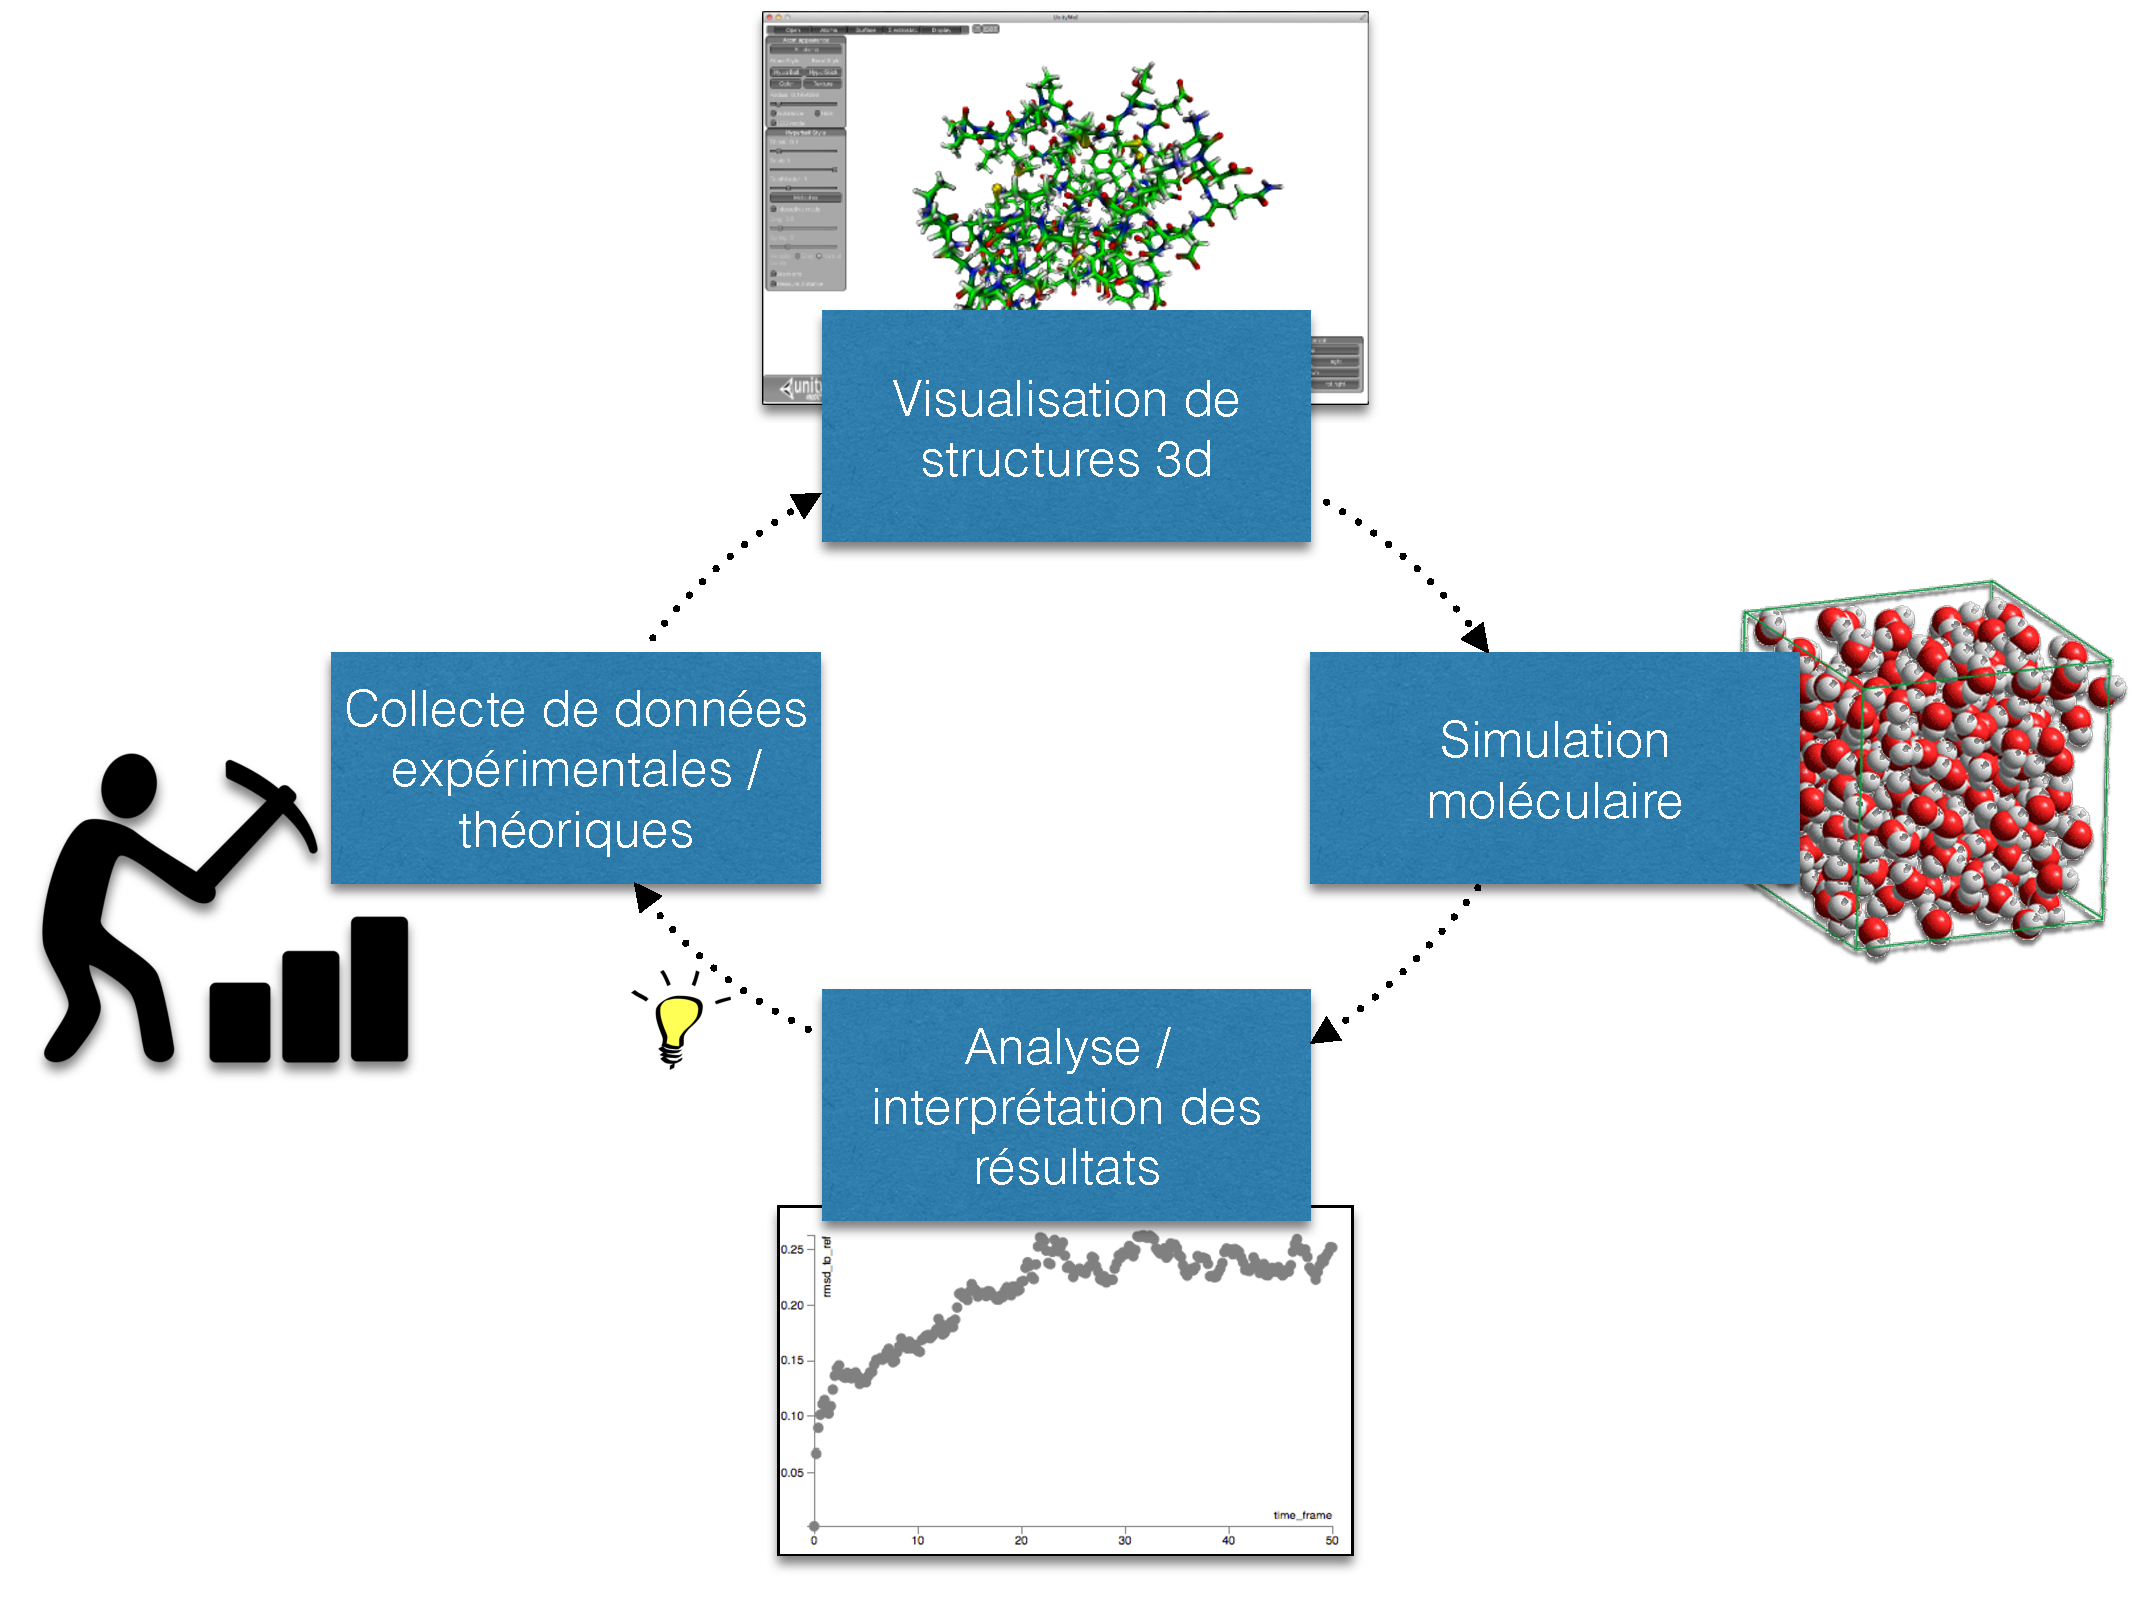
\includegraphics[width=.75\linewidth]{./figures/ch2/ch2_structural_biology_process}}
    \caption{{\it Processus séquentiel standard de l'étude d'un système moléculaire en biologie structurale.}}
  \label{Fig:schema_seq_bio_struct}
  \hspace{0.3cm}
\end{figure}

\section{Analyse post-simulation moléculaire}

Au cœur de la boucle de décision de l'expert en biologie structurale, l'analyse des données de modélisation est donc une étape cruciale, et souvent la plus importante, de la mise en place d'hypothèses scientifiques autour d'un sujet donné. La précision de l'analyse aura une conséquence directe sur la justesse de l'hypothèse émise par l'expert scientifique. Elle nécessite de traiter efficacement la masse de données générée par un processus de simulation ou de modélisation. Dans le cadre de la prédiction de structures 3d, cette analyse peut passer par:

\begin{enumerate}
	\item L'étude énergétique du ou des modèle(s) généré(s) par l'algorithme de modélisation utilisé.
	\item La cohérence des valeurs physico-chimiques associées aux modèles 3d.
	\item La similarité avec de potentiels modèles de familles protéiques proches.
	\item La cohérence biologique des complexes lors de simulation de docking.
\end{enumerate}

Le processus d'analyse n'est pas statique et ne possède aucun caractère universel, il va largement varier suivant le complexe protéique étudié, le type de connaissance recherché et les données générées par les programmes utilisées. La liste précédente reprend donc certaines des approches analytiques les plus courantes mais elle n'est ni exhaustive, ni vouée à constituer un processus immuable d'analyse.

Parmi les processus d'analyse, celui permettant d'analyser une simulation ou dynamique moléculaire est complexe, principalement à cause de son aspect dynamique impliquant l'observation d'un phénomène à travers ses caractéristiques à la fois spatiales mais également temporelles. L'illustration de cette complexité peut se retrouver par exemple dans les différences de niveau d'énergie potentielle retrouvées tout au long de la simulation. Lorsque l'énergie potentielle à un instant précis est élevée, le modèle peut représenter une étape de transition entre deux conformations plus stables mais peut également constituer une structuration non naturelle et le résultat exclusif des contraintes computationnelles. L'évolution de la conformation spatiale de la protéine va donc être d'une grande importante en simulation moléculaire. Même si la finalité sera parfois l'obtention d'un modèle stable en fin de processus, les étapes ayant permis la création de ce modèle ne peuvent être négligées.

Les simulations numériques génèrent, en plus des coordonnées 3d du complexe moléculaire au cours du temps, plusieurs informations importantes pour l'interprétation des évolution structurelles. Ces informations sont pour la plupart des valeurs énergétiques associées à chaque pas de la simulation. Dans le but de préciser la description du système, d'autres valeurs peuvent être générées à partir de ces informations. Cet ensemble de données propres à la simulation doit permettre de comprendre les phénomènes se déroulant au cours d'une simulation. Il est donc crucial de récupérer ces informations, de les structurer et de les lier aux états structurels de la molécule et d'ainsi comprendre exactement les mécanismes impliqués dans les changements structuraux observés.

Au-delà de la simple extraction et lecture des données brutes générées par la simulation, les premières informations pertinentes extraites d'une simulation sont le résultat de la mise en relation des différentes données. L'idée est de corrélée des évolutions temporelles de valeurs pour des données hétérogènes et parfois non liées afin de détecter d'éventuels points remarquables traduisant un phénomène particulier. Divers graphiques, nuages de points ou autres techniques visuelles de mise en relation permettent d'extraire de premières informations précieuses pour la compréhension du déroulement d'une simulation. Ces techniques se couplent particulièrement bien aux analyses eiques de l'évolution conformationnelle d'une structure tout au long de la simulation. Nous avons vu dans les sections \ref{simu_eval} et \ref{docking_eval} que ces analyses sont parfois partie intégrante de l'algorithme régissant le processus d'évolution de la simulation lorsque le \textit{scoring} s'appuie sur des facteurs statistiques pour évaluer la stabilité énergétique d'une structure, en particulier dans les simulations de docking moléculaire.

Les approches analytiques ne passent pas exclusivement par l'analyse stricte des données de la simulation et nous avons vu dans le chapitre précédent (voir section \ref{simu_eval}) qu'il était possible d'évaluer certaines étapes de modélisation grâce des informations statistiques (à différencier de physico-chimiques), rapportant par exemple la stabilité d'une protéine au cours du temps suite à des mutations particulières de sa séquences en acides aminés. Il est parfois donc pertinent de vérifier que les parties conservées au cours de l'évolution sont préservées, de savoir à quel point certaines régions de la protéines varient de leurs homologues et si d'éventuels sites d'action et de liaison sont conservés.
Dans le cas d'analyses de docking, en plus des préoccupations analytiques précédente, la présence de plusieurs molécules censées former une liaison implique des approches supplémentaires. La vérification des contraintes structurales et énergétiques de la protéine respectées après liaison d'un ligand est une étape indispensable, de la même façon que que l'observation d'une modification conformationnelle significative de la protéine entre son état lié et son état non-lié. La stabilité d'un complexe pourra également être reflétée par le nombre de liaisons covalentes ayant été formées, la nature de ces liaisons et leurs contributions énergétiques locale et globale.

Les analyses post-simulation permettant d'extraire des informations de la trajectoire sont souvent intégrées dans la suite d'outils ayant été utilisée pour la simulation (AMBER \cite{pearlman1995amber}, CHARMM \cite{brooks2009charmm}, GROMACS \cite{pronk2013gromacs} pour les plus connus d'entre-eux). Cependant, plusieurs bibliothèques ont également été conçues afin de permettre d'utiliser certains algorithmes et outils d'analyses de simulation moléculaire en dehors des suites logicielles dédiées (BioPython \cite{cock_biopython:_2009}, MDAnalysis \cite{michaud-agrawal_mdanalysis:_2011}, MDTraj \cite{McGibbon2014MDTraj} par exemple).

L'hétérogénéité de ces résultats, de leur nature et de leur impact sur les futures hypothèses scientifiques motivent la volonté de créer un cadre homogène où ces données pourraient être liées et analysées conjointement. 
Différents mécanismes permettent cette homogénéité. La mise en place de repères visuels (codes couleurs ou formes géométriques par exemple) au sein des espaces de visualisation est un premier moyen. Lorsque les données physico-chimiques sont associées à des sous-ensembles de la protéine (hydrophobie des acides aminés, polarité des atomes, distance des atomes au centre de gravité de la protéine, etc.) alors un repère visuel est ajouté à la représentation 3d du sous-ensemble concerné. Les logiciels de visualisation moléculaire intègrent souvent nativement ces standards de représentation même si leur paramétrisation n'est pas souvent directe et passe par un codage spécifique de l'information à afficher au sein de fichiers de coordonnées type PDB. Cette approche permet donc de mettre en relation des informations de manière extrêmement intuitive pour l'utilisateur accélérant ainsi son processus cognitif de fusion des informations.

\section{Visualisation moléculaire 3d} \label{visu_molecular}

Afin de mieux cerner les opportunités d'analyse apportées par la visualisation moléculaire, il semble important d'en préciser les contours et les enjeux actuels.

\subsection{Caractéristiques}

Les programmes de visualisation moléculaire 3d permettent d'observer, dans un espace graphique 3d virtuel, des représentations abstraites de molécules, à partir de fichiers de leurs coordonnées 3d, dont l'extension commune est le PDB.
Ces logiciels permettent principalement de mettre en avant certaines des particularités structurelles des molécules observées via des jeux de couleurs ou de formes largement adoptés dans la communauté et considérés comme des standards. Ces programmes s'appuient sur différents formats de fichier pour ces coordonnées même si la plupart sont capables de lire au moins le format PDB. Au-delà de la visualisation statique de structures 3d, il est souvent possible d'utiliser ces programmes afin de lire la trajectoire d'une simulation numérique. Ainsi, il est possible d'observer l'évolution structurelle d'un complexe moléculaire au cours du temps ou d'observer des phénomènes biologiques (passage de molécules au travers d'une membrane, repliement d'une région protéique suite à son interaction avec un partenaire biologique, etc.). Parmi les programmes de visualisation 3d largement utilisés aujourd'hui nous pouvons citer: 
\begin{itemize}
	\item \textbf{PyMol} \cite{delano_pymol_2002}, basé sur le langage Python et offrant une API pour ce langage, il dispose de nombreux rendus visuels et est, selon l'auteur original, utilisé dans plus d'un quart des images de structures moléculaires présentes dans les articles scientifiques. Il s'appuie sur la génération d'images de haute qualité grâce à des techniques de lancer de rayons.
	\item \textbf{VMD} \cite{humphrey_vmd:_1996}, spécialisé dans la visualisation et l'analyse de résultats de simulations de dynamiques moléculaires, cet outil est très usité du fait de ses nombreuses extensions et la possibilité de le relier à NAMD, un programme de dynamique moléculaire, permettant ainsi d'effectuer des simulations moléculaires interactives. Il est de plus bien adapté au rendu temps-réel de large modèles moléculaires grâce à des méthodes de pixellisation triangulaire directement effectuée sur le GPU.
	\item \textbf{Jmol} \cite{herraez2006biomolecules}, basé sur Java et disponible sous forme d'application indépendante ou intégrée dans des pages web, ce visualiseur est populaire du fait de sa facile intégration au sein de contenus web. Il offre de plus plusieurs rendus graphiques très performants.
	\item \textbf{YASARA} \cite{krieger2014yasara}, suite logicielle permettant à la fois la visualisation mais aussi l’exécution de simulations moléculaires interactives, YASARA est depuis sa création dédiée pour le rendu stéréoscopique 3d et l'implication de l'utilisateur dans le suivi de sa simulation offrant même des solutions pour diriger la simulation en y ajoutant des forces.
\end{itemize}

Cette liste est non-exhaustive mais recense quatre des logiciels de visualisation moléculaire les plus utilisés dans le monde scientifique et plus particulièrement en biologie structurale.

Ces programmes sont tous capables de représenter des modèles 3d de protéines grâce aux standards de représentation mis au point à travers les années. Parmi ceux-ci, il est possible d'extraire 5 modes de représentations souvent utilisés par la communauté de biologie structurale, à la fois dans leur travail quotidien mais également au travers de leurs communications (conférences, articles, etc.).

\begin{itemize}
	\item Représentation par \textbf{ligne}: seuls les liaisons covalentes entre atomes sont représentées par une ligne de longueur équivalente à la distance entre les deux centres des atomes situés de part et d'autre de la liaison. Cette représentation est souvent associée à une coloration précise, chacune de ses moitiés étant colorées de la couleur associée au type d'atome qu'elle relie.
	\item Représentation par \textbf{licorice}: seule la chaîne principale de la protéine est représentée dans ce mode, par des batons droits 
	\item Représentation par \textbf{balles et bâtons}: alors que les atomes sont représentés par des sphères, les liaisons covalentes sont des bâtons.
	\item Représentation par \textbf{rubans}: de la même manière que la représentation par licorice, cette représentation suit les carbones alpha composant la chaîne principale de la protéine et affiche un ruban le long de la chaîne.
	\item Représentation par \textit{\textbf{cartoon}}: ici, les différentes structurations composant la structure secondaire d'une protéine: hélice, feuillet et coude, sont mises en avant respectivement par un ruban enroulé le long du squelette de la protéine, une flèche large pointant dans la direction du feuillet identifié et enfin un tube pour les coudes et boucles de la protéine rassemblant les parties non structurées.
	\item Représentation par \textbf{sphères}: chaque atome est représenté par une sphère dont le rayon est égal au rayon de Van der Waals de l'atome.
	\item Représentation par \textbf{surface}: dans ce mode, la SAS est représentée par une couche uniforme autour de la protéine. 
\end{itemize}

Chaque type de représentation répond à des besoins de visualisation différents. Alors que l'agencement de la structure secondaire et tertiare pourra être rapidement visualisé avec une représentation par \textit{cartoon}, il sera nécessaire d'ajouter une représentation par lignes afin d'observer la proximité des atomes entre eux. De la même façon, la détection visuelle des trous et potentiels sites de liaisons de la protéine sera facilitée par la représentation surfacique mais le cœur de la protéine ne pourra être représenté correctement qu'avec des représentation par ligne ou rubans. Ces différentes représentations ne sont pas cloisonnées et il n'est pas rare de les combiner afin de visualiser les caractéristiques propres à chaque représentation en même temps. Les calculs permettant ces représentations ne demandent pas les mêmes ressources computationnelles et même si la majorité d'entre-elles peuvent aujourd'hui être appliquées de façon presque instantannée sur des ordinateurs de bureau, certaines comme la représentation par surfaces demandent des calculs relativement coûteux sur des protéines de grande taille.

La représentation de surface fait partie des techniques de visualisation ayant pu profité des avancées rapides provenant de certains domaines non scientifiques comme le jeu vidéo ou le cinéma. Certains rendus appelés \textit{photoréalistes} et inspirés de techniques d'animation récentes sont maintenant retrouvés au sein de logiciels de visualisation de données scientifiques, améliorant de façon significative la perception des utilisateurs vis-à-vis de leurs données. La visualisation moléculaire n'a pas échappé à ces nouvelles techniques de rendus et a su implémenté certaines approches basées sur la \textbf{transparence}, les rendus \textbf{lumineux}, les effets de \textbf{profondeur}, etc. au sein des logiciels les plus utilisés dans la communauté. Ces nouvelles façons de représenter des structures protéiques permet de jouer sur les capacités cognitives et perceptuelles des utilisateurs. Parallèlement, ces développements demandant des ressources computationnelles bien plus importantes que les anciennes implémentations graphiques, il a fallu également franchir le pas du calcul graphique sur GPU \cite{chavent_gpu-powered_2011}. La parallélisation des programmes et leur utilisation des ressources graphiques présentes au sein des ordinateurs a permis de conserver des performances d'affichages suffisantes pour afficher des molécules de taille raisonnable. Dans cette même dynamique, certains projets s'appuient sur l'utilisation de moteurs de jeux vidéos pour développer des environnements de visualisation profitant des derniers progrès du domaine, dont la spécialisation et l'investissement associé dépasse de loin les moyens attribués à la seule visualisation moléculaire dans le monde de la science \cite{andrei2012intuitive,lv_game_2013}. Ces moteurs de jeu ouvrent de nouvelles perspectives pour la visualisation mais également l'exploration des structures de protéines.

\subsection{Limites et perspectives}

La présence de GPU performants sur une grande partie du parc informatique scientifique permet d'envisager sérieusement leur utilisation intensive pour le développement d'outils de visualisation performants. La prochaine grande étape est la mise à l'échelle de ces outils pour répondre aux enjeux de taille, au sens propre comme au figuré, inhérents aux structures désormais étudiées. Nous avons vu que ces dernières peuvent maintenant être composées de plusieurs millions d'atomes et donc occupé un espace d'affichage conséquent. Alors que la visualisation de quelques centaines d'atomes sur un écran d'ordinateur de bureau permet d'aborder la structure d'un point de vue détaillé tout en gardant une idée précise de sa structure générale et plus spécifiquement de la position de la caméra par rapport à la protéine affichée, les structures de plus grandes tailles nécessitent une résolution beaucoup plus importante et des moyens d'explorer ces structures de façon contrôlée et sans pertes de repères pour l'utilisateur. Or, parmi les différentes techniques de visualisation évoquées précédemment, si nous pouvons facilement constater les efforts effectués dans le rendu graphiques des protéines, aucune contribution significative n'a été publiée pour les paradigmes de navigation et d'exploration depuis plusieurs années. Ces aspects sont par contre centraux dans les sujets d'étude propres à la RV qui accorde une attention particulière à la place de l'utilisateur au sein des mondes virtuels avec lesquels il interagit \cite{SHOCAM, Hovercam, etc.}.

Ce dernier point, couplé au rapprochement entre les méthodes provenant de disciplines spécialisées dans les rendus visuels de haute performance et l'application scientifique, peut expliquer la progressive arrivée de la visualisation moléculaire dans le monde de la Réalité Virtuelle. Il est d'ailleurs intéressant de constater dans la Figure \ref{Fig:VR_pubmed_trend} le nombre d'articles présent dans la base de données PubMed\footnote{\url{http://www.ncbi.nlm.nih.gov/pubmed}} et comportant le terme "Virtual Reality" dans le titre ou le résumé. Même si ces résultats brutes sont à prendre avec recul, l'évolution croissante de ce terme au sein d'articles biologiques et de médecine semble clairement indiquer un intérêt croissant de ces deux disciplines scientifiques pour la RV.

\begin{figure}
  \centering
  {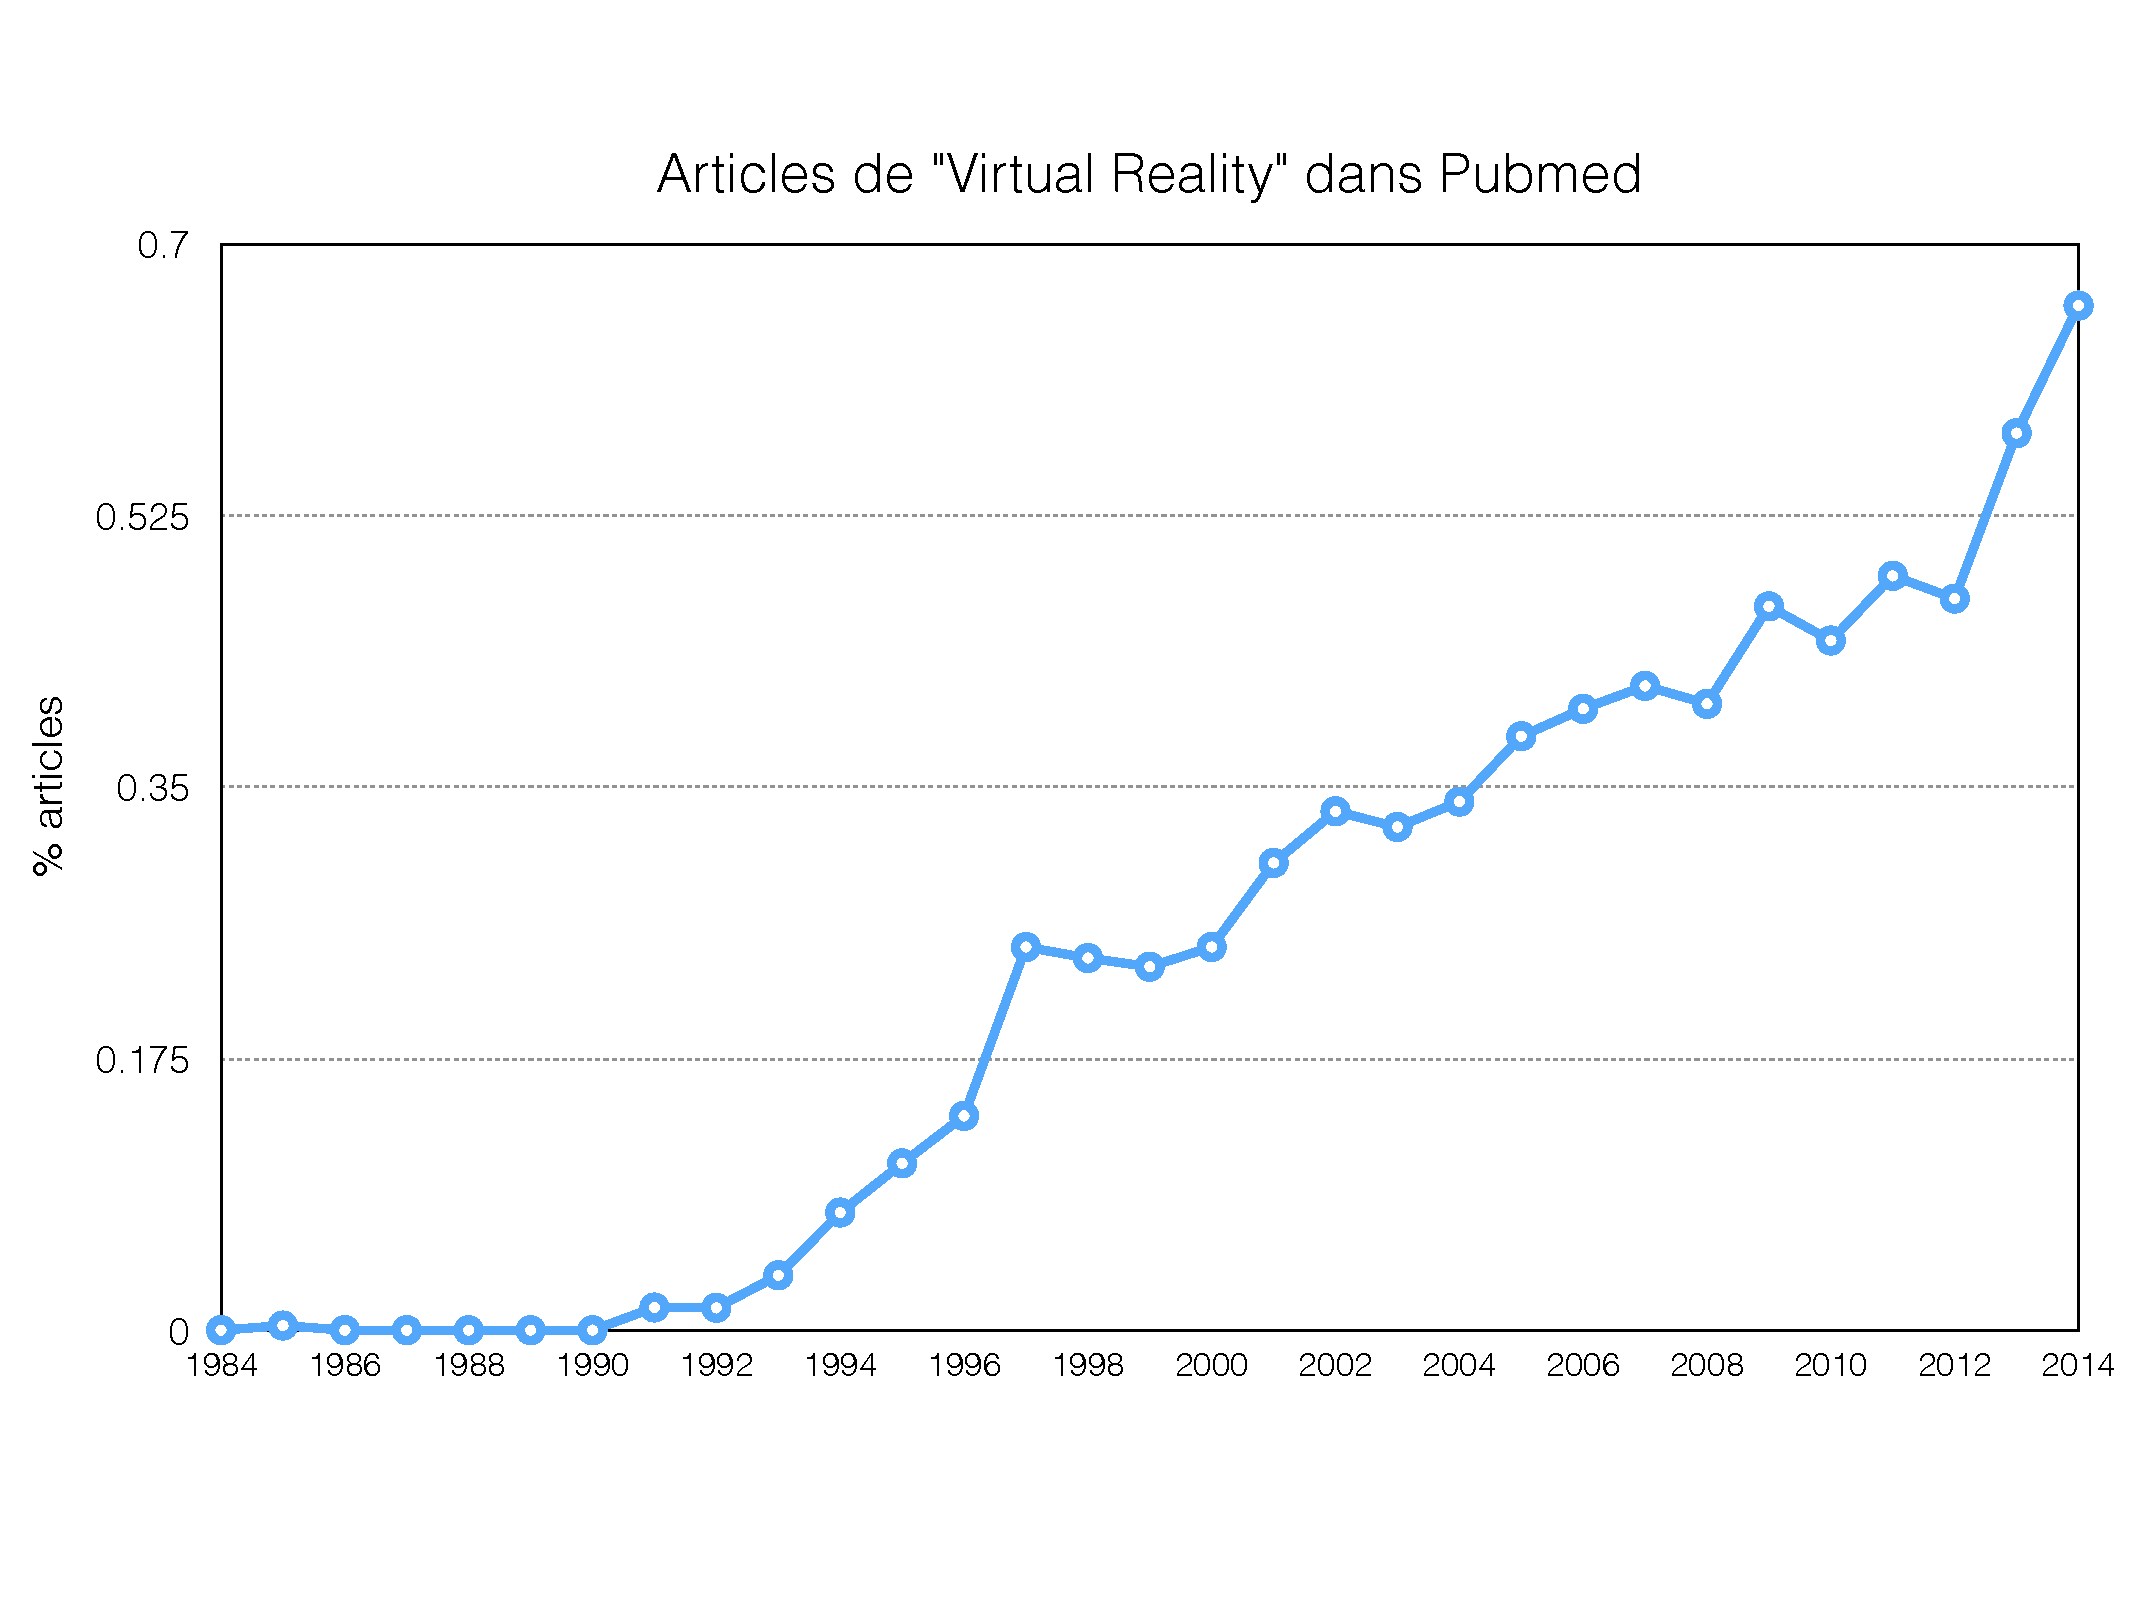
\includegraphics[width=.75\linewidth]{./figures/ch2/VR_pubmed_trend}}
    \caption{{\it Evolution du pourcentage d'articles de PubMed où le terme "Virtual Reality" est retrouvé soit dans le titre soit dans le résumé au cours des 20 dernières années.}}
  \label{Fig:VR_pubmed_trend}
  \hspace{0.3cm}
\end{figure}

\section{Réalité Virtuelle pour la science} \label{RV_science}

La contribution de la Réalité Virtuelle (RV) dans le monde scientifique est en effet relativement récente mais connaît un essor très important depuis quelques années. Cet essor peut être expliquer par deux raisons principales: La démocratisation des dispositifs de réalité virtuelle et augmentée et l'apport de la 3d pour observer des données complexes et/ou intrinsèquement 3d. Comme nous l'avons souligné auparavant, la génération de données est arrivée aujourd'hui à une vitesse haut-débit et dépasse depuis longtemps les capacités d'interprétation de résultats disponibles. Il est donc crucial de trouver un moyen de rapprocher les processus d'analyses des processus de génération de données. Il n'est aujourd'hui pas pensable de réduire la quantité de données générée, il convient donc de mettre en place des solutions d'analyses adaptées, à la fois efficaces et précises et se rapprochant le plus possible des générateurs de données afin d'y filtrer le surplus inutile. La RV, grâce à sa capacité à créer un monde artificiel où les informations peuvent être mêlées entre-elles tout en gardant leur signification est toute adaptée pour répondre au défi de l'optimisation des processus d'analyses.

\subsection{Définitions}

Plusieurs définitions de la RV ont été proposé depuis son émergence dans les années 90. Sherman et Craig définissent la RV comme le fait d'être immergé dans un monde virtuel interactif \cite{sherman2002understanding}. Brooks formule cette définition de manière presque similaire en disant que la RV est une expérience où l'utilisateur est efficacement immergé dans un monde virtuel réactif \cite{brooks1999s}. De façon légèrement différente, Burdea décrit la RV comme une simulation dans laquelle les graphismes générés par informatique sont utilisé pour créer un monde au rendu réaliste qui n'est pas statique mais répond aux sollicitations de l'utilisateur \cite{burdea2003virtual}. On retrouve dans ces définitions les trois piliers qui définissent la RV selon Heim : Immersion, Interaction, Information \cite{heim1998virtual}. Bien qu'il soit difficile d'extraire une définition simple et unique de la RV, l'idée principale est bien de mettre l'utilisateur au centre d'un environnement dynamique et réactif, créé artificiellement et qui viendra supplanter le monde réel le temps de l'expérience. Ceci est très proche de la définition de la RV que nous considérons au sein de l'équipe VENISE du LIMSI-CNRS \cite{bourdot_patrick_reconstruction_2002}:

\textit{La Réalité Virtuelle vise à mettre au point des systèmes informatiques qui donnent à l'humain la capacité de percevoir et d’interagir de façon multi-sensori-motrice avec des données numériques ou mondes virtuels. Quand en plus, ces données numériques intègrent une virtualisation d’une partie de l’univers réel et permettent ainsi de gérer des interactions entre des objets totalement virtuels et des objets réels, on parle alors de Réalité Augmentée, voire de Réalité Mixte.
}

L'immersion de l'utilisateur passe par la mise en place de retours sensoriels précis et réalistes qui vont amener l'utilisateur à considérer le monde virtuel comme un monde plausible. L'interaction est donc primordiale puisqu'un utilisateur va attendre de la part du monde dans lequel il évolue un retour d'information répondant à ses actions. Ces retours d'informations peuvent être de différentes formes, souvent visuels, ils peuvent en fait s'adresser à l'ensemble des sens de l'utilisateur. C'est la richesse de ces retours qui définira le degré d'immersion de l'utilisateur et donc son implication dans le monde virtuel. Bowman et McMahan notent qu'il n'est cependant pas nécessaire de gérer l'ensemble des sollicitations sensorielles d'un utilisateur pour assurer une immersion acceptable \cite{bowman_virtual_2007}. Dans cette même étude, les auteurs proposent un découpage de l'immersion en plusieurs composants, invoquant une immersion qui n'est jamais soit absente, soit parfaite. Ils vont même plus loin en évoquant les applications de RV où la présence de l'utilisateur n'est pas primordiale. Dans ces applications, la perception du monde virtuel et de son contenu passe avant la sensation de présence de l'utilisateur. Parmi ces applications, la visualisation de données scientifiques, qui nous intéresse dans notre étude, met davantage l'accent sur le contenu que sur l'effort pour immerger l'utilisateur dans un monde virtuel.

\subsection{Dispositifs immersifs de RV}

Il est difficile de décrire la RV sans décrire les dispositifs qui lui servent de support. Conçu pour solliciter l'ensemble des canaux sensorimoteurs de l'homme, ces dispositifs doivent permettre à l'utilisateur de percevoir le monde virtuel dans lequel il évolue le mieux possible afin qu'il y interagisse de la façon la plus adaptée et efficace.
Afin de répondre à chacun des pré-requis que l'immersion génère, il est possible de distinguer 3 types d'interfaces comportementales venant exploiter la motricité ou les perceptions de l'homme issues de son comportement dans le monde réel.
Nous retrouvons: les \textit{interfaces sensorielles} qui vont permettre à l'homme de percevoir le monde virtuel, les \textit{interfaces motrices} qui vont permettre à l'homme d'évoluer et agir dans le monde virtuel et enfin les \textit{interfaces sensori-motrices} qui vont permettre la communication bi-latérale entre l'homme et le monde virtuel.
Nous ne donnerons pas une liste exhaustive des dispositifs de RV mais une telle liste est présente dans le Traité de la Réalité Virtuelle - Volume 2. \cite{fuchs2006traite}.

\subsubsection{Interfaces sensorielles} \label{interface_sensor}

Parmi les interfaces sensorielles, il n'est pas abusif de dire que les interfaces visuelles sont les plus importantes en RV. Elles sont de loin les plus utilisées pour l'immersion et bien que d'autres interfaces sont également utilisées dans des cas ponctuels, elles le sont rarement sans couplage à des interfaces visuels.

\paragraph{Stéréoscopie ou rendu 3d}

On ne peut évoquer les interfaces visuelles immersives sans s'arrêter sur le concept de stéréoscopie, à la base de l'intégralité de ces interfaces. La stéréoscopie se caractérise par la génération de deux images distinctes, une par oeil, avec un décalage minime de point de vue. Lorsque chaque image est présentée à l'oeil correspondant, le cerveau traite ces images afin de nous faire percevoir de la profondeur et voir en relief. Il est possible de générer ces images de différentes manières mais dans notre cas, nous travaillons avec des images générées par ordinateur. Ces images sont restituées par un écran ou un projecteur mais doivent ensuite être séparées afin d'attendre indépendamment les deux yeux. Cette séparation peut se faire soit de façon active, soit de façon passive. Lorsque la séparation est active, on occulte la vision des deux yeux de manière alternée et à haute fréquence. Il est donc nécessaire d'afficher la bonne image pour le bon oeil au moment où celui-ci n'est pas occulté. Il existe donc une forte synchronisation entre le générateur d'images et la lunette à occultation utilisée.
Dans le cas d'une séparation passive des images, on utilise un filtre polarisant à la fois sur les écrans et les lunettes. Les deux images sont ici affichées en même temps mais selon deux polarités différentes.

\paragraph{Dispositifs fixes} \label{dispo_fix}

Parmi les dispositifs fixes utilisés en RV on retrouve les murs d'écrans. Evolution naturelle des écrans d'ordinateur classiques, ce sont de larges surfaces composés de plusieurs écrans aux bords fins collés les uns aux autres. Les écrans sont de différentes natures, même si tous les écrans d'un même mur sont identiques, ils peuvent être rétro-projetés ou non, 2d ou 3d, tactiles ou non et de résolutions différentes. Ils permettent l'affichage de larges images à de hautes résolutions et sont souvent utilisés pour les études scientifiques mettant en jeu de nombreuses données à des échelles très différentes.

L'immersion atteint un niveau supérieur lorsque sont utilisés des environnements immersifs de type CAVE \cite{cruz-neira_cave:_1992} comme illustré dans la Figure \ref{Fig:eve_cave_system}. Le système CAVE consiste en une série de projecteurs permettant la projection d'images sur 3 à 6 faces d'un cube de la taille d'une pièce. Les projecteurs peuvent être remplacés par des écrans plats dans certains cas mais cette configuration est plus rare car bien plus coûteuse à taille d'écran similaire. Bien qu'il n'existe pas de tailles limites inférieures ou supérieures lorsqu'on évoque la taille des CAVEs, il est commun de pouvoir s'y tenir debout et donc d'y évoluer. Les projecteurs sont usuellement situés derrière les écrans afin de ne subir aucune entrave dans le rayon de projection. Le contenu affiché est bien souvent 3d et de haute résolution. Les utilisateurs portent des lunettes 3d pour percevoir la stéréoscopie et leurs mouvement sont généralement capturés par des caméras infrarouges grâce à des cibles de petites tailles qu'ils portent sur les lunettes, système que nous détaillerons dans la section \ref{interface_motor}. Il est possible dans un CAVE d'afficher des objets virtuels flottants autour desquels l'utilisateur pourra se déplacer.
Il n'est pas rare de voir des systèmes audio 3d associés aux CAVEs. Ces systèmes audio profitent du large espace de la pièce pour disposer de multiples enceintes.
L'avantage des CAVEs est leur taille et la possibilité de se déplacer dans un monde virtuel de taille raisonnable simplement en marchant. L'intégration de dispositifs d'interaction est également facilitée par la contrainte de taille limitée. 
Certaines CAVEs utilisent plus d'un projecteur par écran leur permettant d'afficher des images pour deux points de vue distincts, en 3d et simultanément, c'est le cas d'EVE\footnote{\url{http://www.limsi.fr/venise/EVEsystem}} (Evolutive Virtuel Environments) du groupe VENISE du LIMSI-CNRS. La multi-stéréoscopie permet de mettre en place des scénarios collaboratifs entre les utilisateurs partageant la même scène virtuelle mais selon leur propre point de vue.

\begin{figure}
  \centering
  {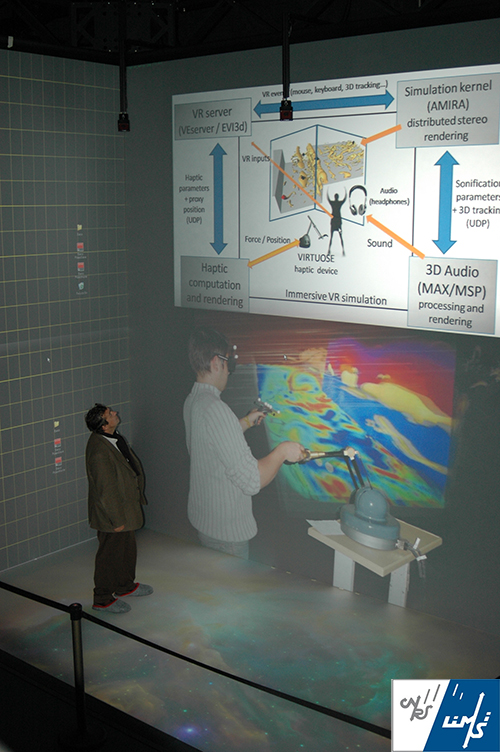
\includegraphics[width=.35\linewidth]{./figures/ch2/eve_cave_system}}
    \caption{{\it Photo de EVE, système CAVE présent au LIMSI/CNRS.}}
  \label{Fig:eve_cave_system}
  \hspace{0.3cm}
\end{figure}

\paragraph{Dispositifs mobiles} \label{dispo_mobil}

Les visiocasques (appelés également casques immersifs ou casques de RV ou encore casques HMD for \textit{Head-Mounted Display} en anglais) sont des dispositifs se portant à la manière de casques standards et composés de deux écrans situés en face des yeux de l'utilisateur. Grâce à un système de lentilles, l'utilisateur est capable de distinguer les images affichées sur chacun des écrans de façon nette. L'affichage peut être soit monoculaire et donc perçu en 2d, soit binoculaire et donc perçu en 3d. Dans ce dernier mode, le contenu affiché sur les écrans est découpé de telle sorte que chaque œil perçoit une image différence correspondant au point de vue qui devrait être le sien dans la réalité comme illustré dans la Figure \ref{Fig:pymol_stereo}. Le contenu affiché évolue suivant l'orientation de la tête de l'utilisateur. Cela est rendu possible par la présence d'un gyromètre calculant l'orientation relative de la tête par rapport à un point d'origine calibré au début de l'expérience. L'utilisateur possède donc une vue sur un contenu virtuel à 360 degrés qu'il peut regarder de la même façon que s'il se trouvait sur une chaise statique mais tournant à 360 degrés. Bien que les premiers visiocasques binoculaires commercialisés datent de 1995, le domaine des casques immersifs a connu depuis quelques années un intérêt significatif de la part du monde de la recherche et du jeu vidéo. Cet intérêt peut s'expliquer par la résolution atteinte par les écrans de petite taille (type smartphone) et la précision des capteurs d'orientation utilisés pour adapter l'image à l'orientation de l'utilisateur. Du point de vue du coût, ces dispositifs sont très peu onéreux comparés aux systèmes fixes. Cependant, l'un de leurs inconvénient est le fait qu'il dissocient l'utilisateur du monde extérieur, favorisant une utilisation solitaire.

\begin{figure}
  \centering
  {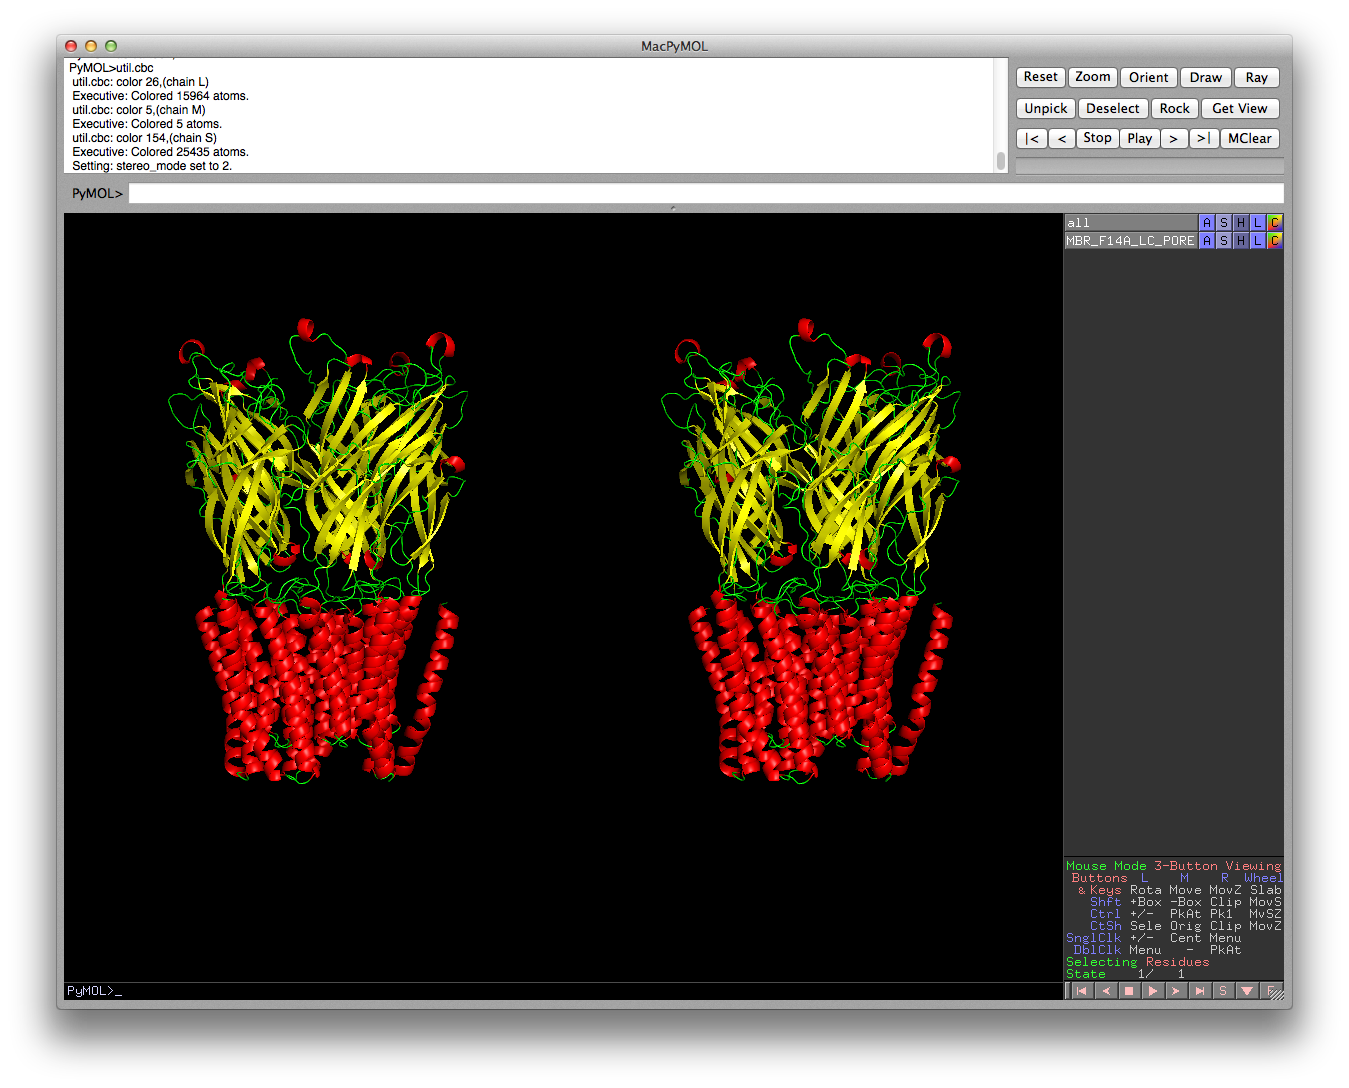
\includegraphics[width=.75\linewidth]{./figures/ch2/pymol_stereo}}
    \caption{{\it Capture d'écran de PyMol exécuté en mode stéréoscopique "cross-eyes": l'image de la protéine de droite correspond à l'oeil gauche et inversement.}}
  \label{Fig:pymol_stereo}
  \hspace{0.3cm}
\end{figure}

\subsubsection{Interfaces motrices} \label{interface_motor}

Afin de se mouvoir et d'évoluer dans le monde virtuel, l'utilisateur doit pouvoir être positionné par la plateforme de rendu. La navigation dans un environnement virtuel est une problématique cruciale en RV, d'autant plus lorsqu'elle s'effectue au sein d'un environnement virtuel abstrait et en l'absence des repères spatiaux habituellement rencontrés dans le monde réel.
Parmi les dispositifs permettant de récupérer les positions de la tête ou du corps de l'utilisateur, le \textit{tracking} optique est l'un des plus usité. Il fonctionne au moyen de caméras infra-rouge et de marqueurs réfléchissants (voir Figure \ref{Fig:ir-tracking}). Des motifs de marqueurs vont servir de cibles pour les caméras infra-rouge qui vont opérer une triangulation afin d'en extraire leur position. Chaque motif différent peut être associé à un objet particulier, une partie du corps ou un dispositif d'interaction. Le suivi de la tête est particulièrement utile dans les environnements immersifs puisqu'il permet de connaître la position et l’orientation de la tête et donc du regard au sein du monde virtuel. Grâce à cela, les ordinateurs responsables du rendu graphiques peuvent adapter les images affichées sur les écrans pour qu'elle corresponde au point de vue de l'utilisateur dans le monde virtuel.
Il est également commun d'utiliser le système de \textit{tracking} afin de capturer les gestes de la main afin de mettre en place des interactions précises avec l'environnement. L'interaction par capture peut également se faire au travers de dispositifs d'interaction de nature variée suivant l'activité exécutée en RV. Parmi ces outils spécifiques, la souris 3d également appelée \textit{flystick} ou la manette de jeu sont couramment utilisés dans les environnements immersifs.
Enfin, il est possible de capturer l'ensemble du corps d'une personne afin de mettre en mouvement sa représentation virtuelle, appelée avatar. L'ensemble des marqueurs vont être répartis sur une combinaison afin d'obtenir la position de l'ensemble des parties mobiles du corps. Cette technique est beaucoup utilisée dans le monde du cinéma par exemple afin d'animer les avatars présents dans les films d'animation. Elle est également utilisée dans la recherche lorsque la perception de soi ou d'un collaborateur est important pour la tâche à effectuée, par exemple au cours d'études ergonomiques.

\begin{figure}
  \centering
  {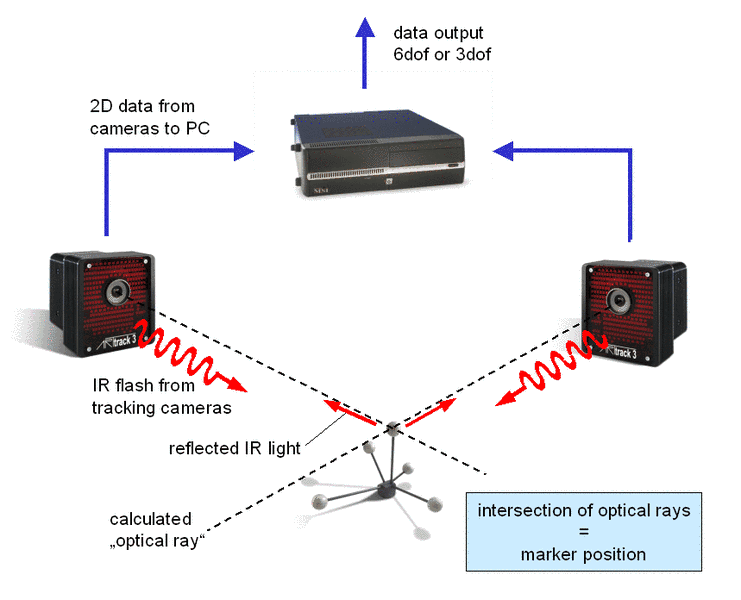
\includegraphics[width=.65\linewidth]{./figures/ch2/IR-tracking}}
    \caption{{\it Schéma simplifié d'un système de tracking optique basé sur des signaux infrarouges lancés par des caméras et se reflétant sur des marqueurs spécifiques. La configuration spatiale des marqueurs est reconnue par le PC et la position associée est calculée à partir des intersections de rayons infrarouges reflétés.}}
  \label{Fig:ir-tracking}
  \hspace{0.3cm}
\end{figure}

\subsubsection{Interfaces sensori-motrices} \label{interface_sensor-motor}

Lorsque la communication entre l'utilisateur et l'environnement est bi-latérale, nous parlons d'interfaces sensori-motrices. Ces interfaces regroupent les dispositifs permettant à la fois d'interagir avec l'environnement mais également de recevoir un stimuli sensoriel en réponse. La plus commune des interfaces sensori-motrices est l'interface haptique qui va permettre à l'utilisateur de ressentir l'effet de son interaction. Les bras à retour d'efforts permettent par exemple de manipuler des objets en 3d tout en ressentant leur poids ou d'éventuelles collisions avec d'autres objets. Le domaine médical et plus généralement des opérations robotisées profitent de ces dispositifs afin de garantir un ressenti tactile complémentaire à l'information visuelle parfois limitée et/ou non suffisante.

\subsubsection{Interactions naturelles et directes} \label{interface_nature}

Afin d'augmenter la sensation d'immersion de l'utilisateur et améliorer son expérience, il existe des interfaces dites naturelles ou directes qui vont chercher à s'inspirer des techniques d'interactions du monde réel. Le premier apport de ces interfaces est qu'elle s'adresse davantage à l'intuition de l'utilisateur que les interfaces évoquées précédemment.
Les interactions directes, regroupant les interactions mettant en jeu des mouvements de l'utilisateur ou des commandes vocales pour interagir avec son environnement virtuel, font opposition aux interactions indirectes comme peuvent l'être le clavier, la souris ou les dispositifs d'interaction immersifs comme la souris 3d ou les manettes évoquées précédemment. Ces méthodes induisent une présence moins importante des menus, favorisant ainsi davantage l'immersion. Il est bon de noter que ces interactions ont souvent une courbe d'apprentissage plus longue que les interactions indirectes. De plus, elle demande souvent une précision plus importante et sont donc soumises à des variations d'efficacité parfois plus importantes. Elles sont cependant moins contraignantes pour l'utilisateur puisqu'elles ne se basent pas sur une charge matérielle autre que des supports de marqueurs pour la capture de gestes et un micro déporté ou non pour la reconnaissance vocale.

La combinaison des différentes méthodes d'interaction que nous avons vu est un domaine de recherche à part entière \cite{martin_hardware_2014,martin_reconfigurable_2011}. On parle de \textbf{multimodalité} lorqu'on propose aux utilisateurs des interactions au travers de leurs différents canaux sensori-moteurs.

\subsection{La RV pour en biologie structurale}

La RV possède plusieurs facettes répondant naturellement aux problèmes posés par l'analyse scientifique. Rappelons la problématique actuelle de la visualisation de données scientifiques. Les données générées excèdent de loin les capacité d'interprétation disponibles. De plus, la complexité et la quantité des données est telle que leur rendu 2d ou 3d sur des écrans d'ordinateur ne sont plus suffisants pour rapporter l'ensemble des informations que les données contiennent. L'accès à certaines informations est donc entravée et enfouie sous la quantité de données à analyser par l'utilisateur.

\subsubsection{Stéréoscopie 3d et perception humaine}

Dans le cadre de la visualisation scientifique, on peut considérer que la capacité d'affichage stéréoscopique doublé à une surface d'affichage à 360 degrés est la facette la plus importante de la RV. Plusieurs études ont par exemple démontré que la perception de la profondeur lors de la représentation de structures moléculaires apportait une aide non négligeable pour leur compréhension structurelle \cite{van_dam_immersive_2000,stone_immersive_2010,odonoghue_visualization_2010}. Les complexes moléculaires et les protéines sont par nature structurées en 3d et c'est cette structuration qui est au cœur des études en biologie structurale. La stéréoscopie est donc une alternative naturelle pour l'observation de structures protéiques puisqu'elle utilise la compréhension innée de la 3d du cerveau humain pour analyser des phénomènes et objets de nature 3d. 
Mais l'étude de la structure seule ne peut suffire lors de l'étude d'un complexe moléculaire, nous avons souligné auparavant la présence de nombreuses données accompagnant la génération de modèles 3d lors d'une simulation moléculaire. Ces données, sous forme de valeurs brutes, doivent être également analysées. La dimension de profondeur propre à la stéréoscopie prend une nouvelle fois tout son sens ici. Ce n'est plus la nature 3d même des données observées qui va rendre cette profondeur importante, puisque nous nous intéressons maintenant à des valeurs numériques brutes, mais la possibilité d'utiliser une 3e dimension pour représenter des modèles, des tendances ou bien des anomalies au sein des données affichées.
Au delà de la stéréoscopie, la surface, ou davantage le volume quand on parle de 3d, disponible dans les dispositifs de RV pour afficher des informations est beaucoup plus important que ce qu'on peut retrouver au sein de dispositifs 2d standards. Combiné avec un suivi de l'orientation et de la position de la tête de l'utilisateur, il devient aisé de créer un monde composé de 360 degrés d'informations accessibles simplement et rapidement au moyen d'un simple coup d'oeil.

\subsubsection{Interfaces sensori-motrices comme vecteurs d'informations}

La notion d'interaction n'intervient pas que dans un sens unique et même si la méthode permettant d'interagir avec un objet est primordiale, le retour sensoriel provoqué par l'interaction est, en RV, un sujet d'étude à part entière. Nous avons vu que ces retours sensoriels participent à l'immersion ressentie par l'utilisateur dans un monde virtuel mais ils peuvent également servir de repères ou de vecteurs d'informations utilisés pour compléter les informations visuelles. Même s'il est possible de mettre en place certaines sollicitations autres que visuelles lors d'un travail sur un poste de travail standard, il est très rare de trouver des retours sonores ou haptiques lors d'une session de travail. Au delà des limites matérielles qui peuvent exister, un retour haptique impliquant par exemple la nécessité de posséder un dispositif muni d'un système de retour d'effort, les limites sont souvent logicielles, peu de programmes implémentent des retours sensoriels autres que visuels dans le design de leurs outils d'analyses de données. Il est au contraire très commun de prendre en compte ces retours sensoriels lors du développement de solutions logicielles dédiées à la RV. La RV est par essence définie par l'implication de l'utilisateur. Il a donc dû développer très tôt des moyens pour retranscrire un maximum de sensations aux utilisateurs lors de leurs expériences virtuelles. En visualisation de données abstraites et/ou scientifiques, l'utilisation de méthodes de retours sensoriels a pu ensuite être détourné de leur but premier, l'immersion, pour communiquer des informations supplémentaires à l'utilisateur pendant ses phases d'interactions. La possibilité par exemple de déclencher un événement sonore lors de la sélection de données critiques ou extrêmes dans un set de données est l'un des exemples de l'utilisation d'un retour auditif pour transmettre une information \cite{ferey_multisensory_2009}. De la même façon, le domaine de la conception assistée par ordinateur (CAO), très présent en RV, utilise des dispositifs de retour de force afin de juger de la résistance de matériaux ou de limites de torsion/translation des objets \cite{sun2010haptic}. La chirurgie est également demandeuse de solutions précises de retours haptiques au sein de ses récentes applications de RV dédiées à l’entraînement des chirurgiens à des opérations spécifiques ou développées pour le contrôle de robots pour des opérations sur des patients réels \cite{kusumoto_application_2006}. Étendre ces moyens de fournir des informations par d'autres canaux que les canaux visuels pour la visualisation de données scientifiques en RV est donc une solution réaliste et concrète, simplifiée par les méthodes de RV déjà existantes.


\subsubsection{Applications}

La biologie structurale n'a su que tardivement se placer par rapport à la RV. Ce n'est que très récemment que certains programmes dédiés à l'exploration moléculaire ont commencé à être utilisé au sein de dispositifs de RV \cite{odonoghue_visualization_2010}. YASARA \cite{krieger2014yasara} ou VMD \cite{stone_immersive_2010} sont deux exemples de programmes de visualisation moléculaires disponibles pour un rendu stéréoscopique et adapté aux environnements immersifs. Ils permettent l'interfaçage de leur solution de visualisation avec de nombreuses librairies utilisées en RV dans les systèmes immersifs de type CAVE ou mur d'écran. Nous pouvons citer VRPN \cite{taylor2001vrpn}, FreeVR \cite{pape2004commodity} ou VR Juggler par exemple, 3 suites de librairies. 
D'autres initiatives ponctuelles ont aussi vu le portage d'autres logiciels dans des environnements immersifs mais ces développements spécifiques ont rarement dépassé l'extension du rendu graphique depuis le 2d jusqu'en 3d\footnote{\url{http://www.rug.nl/science-and-society/centre-for-information-technology/research/hpcv/vr\_visualisation/mol\_visualisation?lang=en}} ou la mise en place de librairies comme base de développement d'applications RV pour la visualisation moléculaire \cite{salvadori_moka:_2014}.  Afin d'améliorer l'apprentissage de certains concepts biologiques, il est parfois utile d'en améliorer la perception, en particulier quand ces concepts sont par aspects abstraits. Un projet éducatif a cherché à évaluer l'impact pour les étudiants de visualiser des objets moléculaires en RV dans le cadre de cours de biologie structurale \cite{tan_use_2013}. Selon leurs conclusions, les dispositifs immersifs ont permis un meilleur apprentissage des notions abordées ainsi qu'une compréhension globale de la biologie structurale plus complète.
La liste des applications mêlant explicitement la biologie structurale et la RV est relativement courte. Le travail d'ingénierie est par aspects déjà fait mais il semble manquer une réflexion ergonomique autour de l'intégration des outils de biologie structurale au sein de dispositifs immersifs. 

Une première pierre pour cette réflexion pourrait venir, selon nous, du domaine de la visualisation analytique et de ses problématiques, parfois proches de celles que nous retrouvons en RV.
Lorsque l'on s'intéresse à la place de la visualisation analytique dans les disciplines de biologie et de médecine (voir Figure \ref{Fig:VA_pubmed_trend}), on s'aperçoit que la visualisation analytique connaît une progression identique à celle de la RV. Il est possible d'expliquer cette croissance par la nécessité de trouver des algorithmes de visualisation adaptés aux données manipulées aujourd'hui.

\begin{figure}
  \centering
  {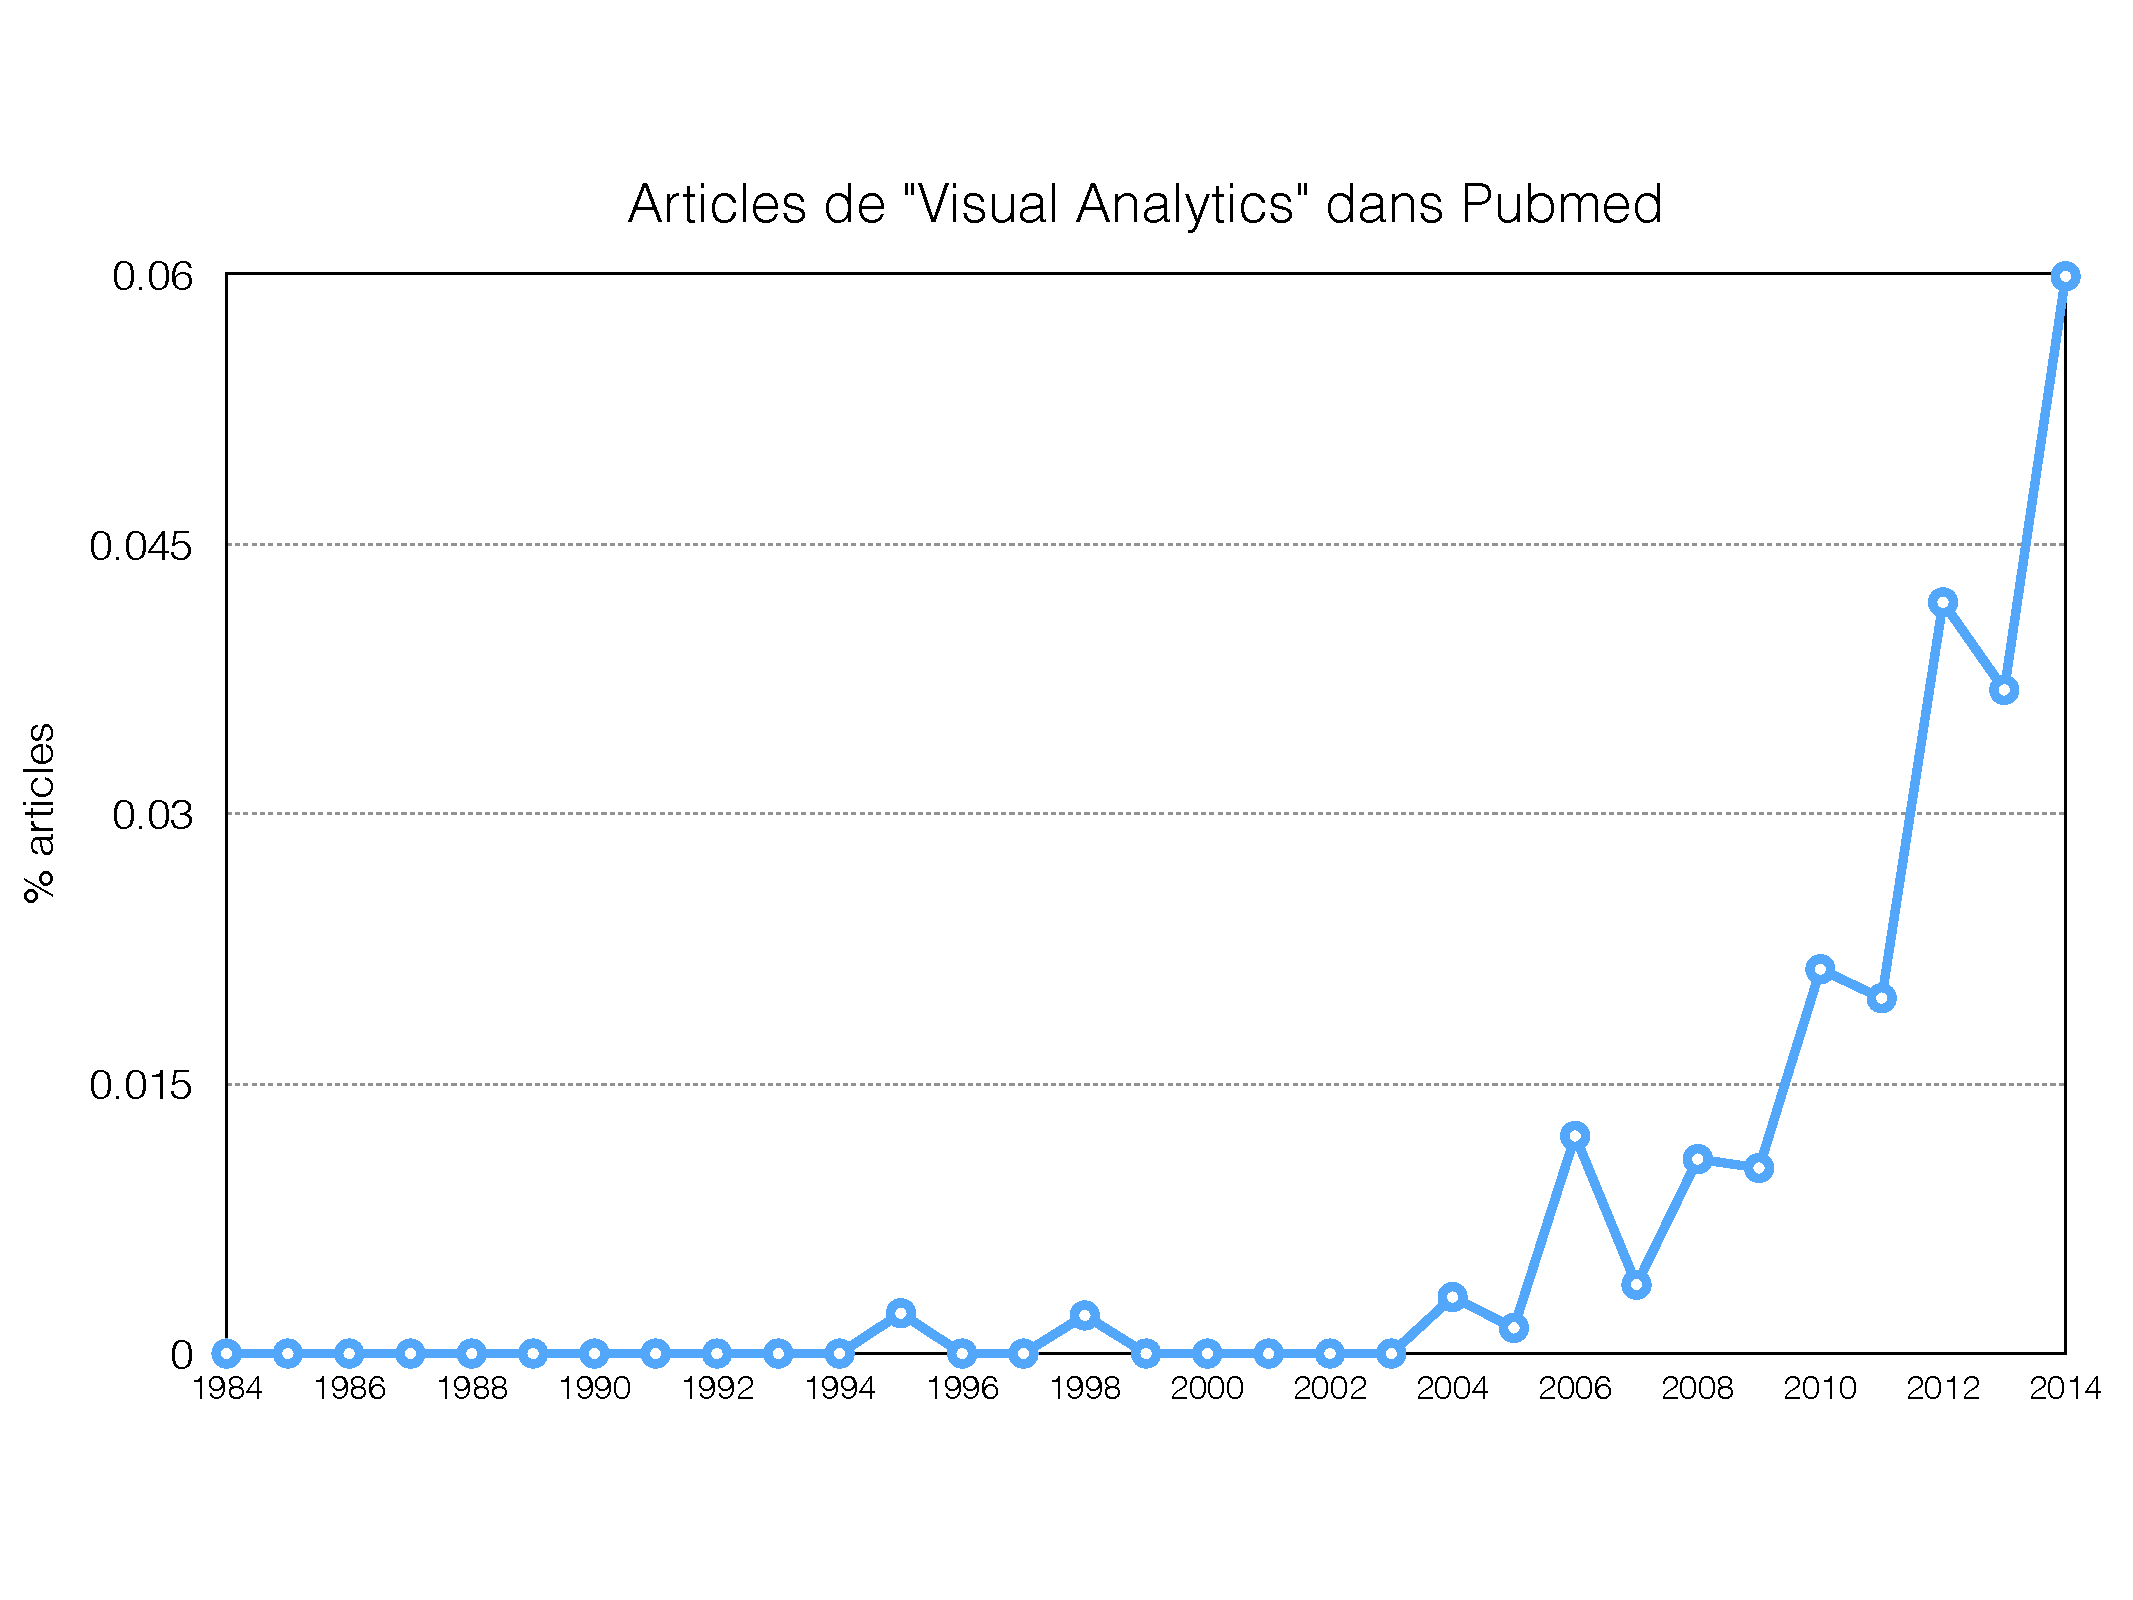
\includegraphics[width=.75\linewidth]{./figures/ch2/VA_pubmed_trend}}
    \caption{{\it Evolution du pourcentage d'articles de PubMed où le terme "Visual Analytics" est retrouvé soit dans le titre soit dans le résumé au cours des 20 dernières années.}}
  \label{Fig:VA_pubmed_trend}
  \hspace{0.3cm}
\end{figure}


\section{Visualisation analytique}

L'association étroite entre la visualisation d'informations scientifiques et les analyses associées, dans un même espace et simultanément, met en avant des techniques de visualisation connues et souvent définies en visualisation analytique.

\subsection{Définition}

Cette discipline récente a en effet pour but de faciliter l'analyse visuelle de données complexes et/ou scientifiques et se définie par le "raisonnement analytique au travers d'interfaces visuelles interactives" \cite{cook_illuminating_2005}. Elle se place à la frontière de nombreux domaines de visualisation, d'interaction ou de perception afin de mettre en avant des informations qui n'auraient pu apparaître lors de l'utilisation cloisonnée des différents domaines mis en jeu. La visualisation analytique s'appuie sur des méthodes de visualisation simples et compréhensibles par l'être humain auxquelles elle ajoute une dimension interactive afin de les relier entre elles. Elle s'inspire donc par plusieurs niveaux aux études d'interactions homme-machine (IHM) dont la réalité virtuelle s'inspire également \cite{arias-hernandez_visual_2011}. De la même manière qu'en IHM, elle se repose sur des outils et des techniques basées sur des considérations ergonomiques et perceptuelles. Son principal but est de mettre l'être humain au centre d'une boucle de décision qui sera facilitée par la mise en relation de données de différentes natures et de différentes sources. Ce contexte de travail généré par la visualisation analytique doit être cohérent pour le chercheur. C'est à ce niveau que les domaines de la perception et des études cognitives interviennent afin d'assurer une pleine compréhension et utilisation de l'espace de travail. La VA se place comme un catalyseur de domaines comme le raisonnement analytique, l'interaction, la transformation et la représentations des données pour leur visualisation et analyses.
Elle a par beaucoup de facettes des points communs importants avec la \textbf{visualisation d'information} et la \textbf{visualisation scientifique}. Leurs limites respectives et leurs frontières sont assez floues mais elles peuvent être distinguées de la manière suivante:

\begin{itemize}
	\item \textbf{La visualisation scientifique} s'intéresse aux données possédant une structure géométrique 3d native (images médicales, évolution de fluides, structures atomiques par exemple).
	\item \textbf{La visualisation d'informations} se tourne elle vers la représentation de données abstraites comme les graphiques ou les réseaux de données.
	\item \textbf{La visualisation analytique} est davantage concernée par le couplage de représentations visuelles interactives avec des processus analytiques afin d'extraire de nouvelles informations.
\end{itemize}

\begin{figure}
  \centering
  {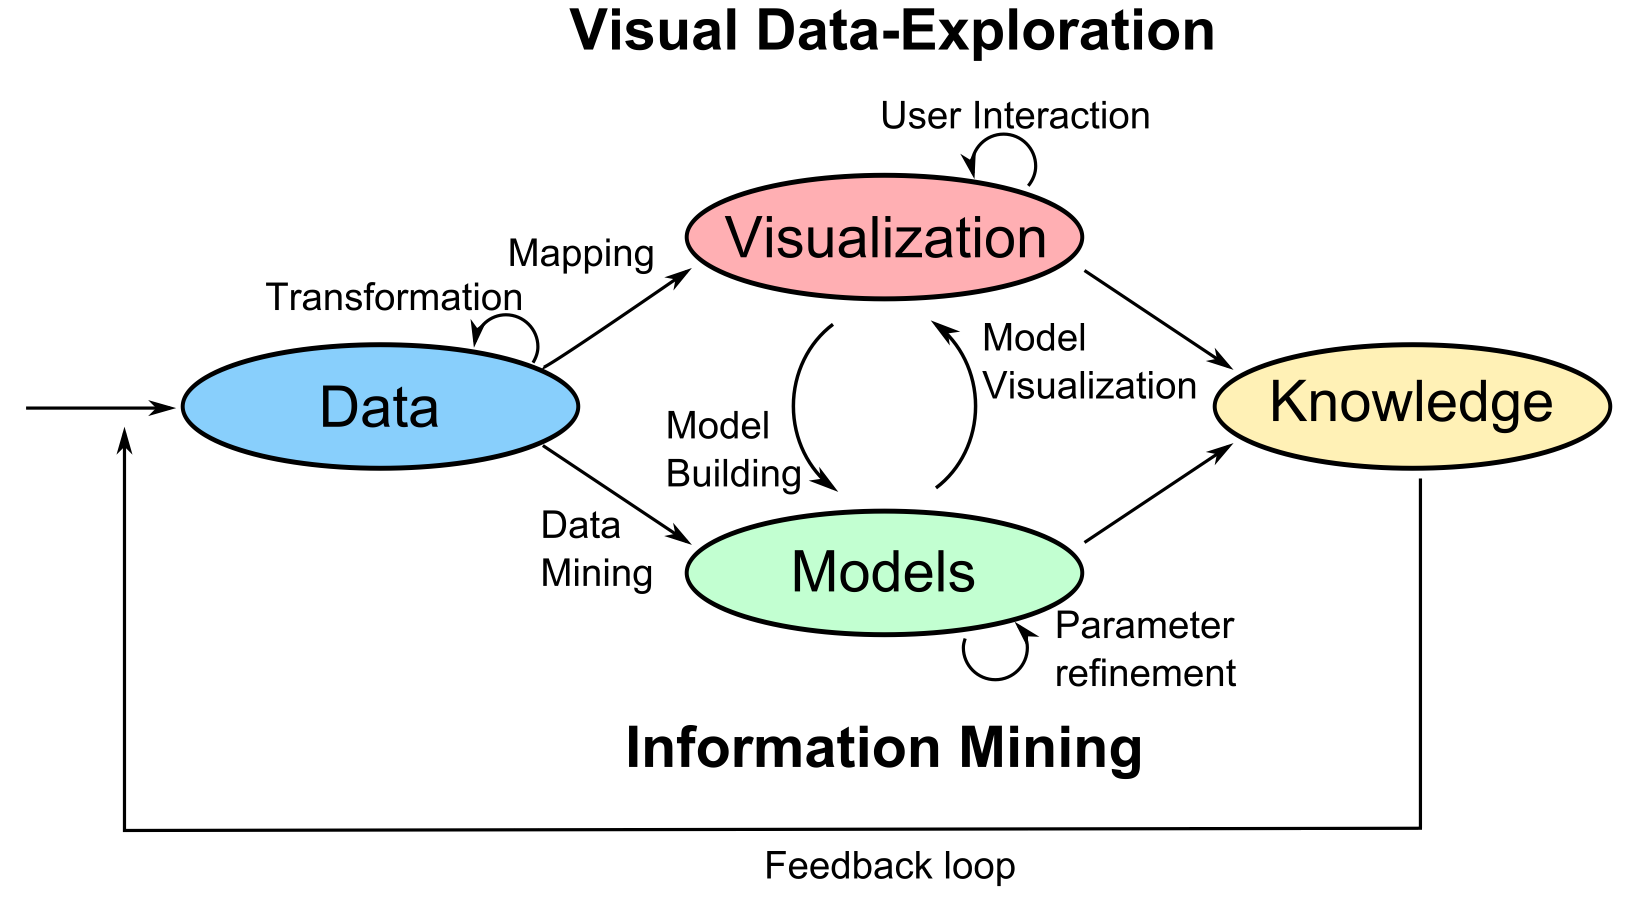
\includegraphics[width=.75\linewidth]{./figures/ch2/visual_analytics_process_keim}}
    \caption{{\it Schéma illustratif du processus de Visual Analytics tel que proposé par Keim \textit{et al.}. Les différentes étapes sont illustrées par des ovales, les transitions par des flèches.}}
  \label{Fig:visual_analytics_process_keim}
  \hspace{0.3cm}
\end{figure}

La visualisation analytique vise donc à combiner la visualisation de données passées en entrée et leurs analyses afin de créer de nouvelles connaissances qui pourront elles-mêmes être utilisées par la suite en entrée de la boucle. Ce processus, expliqué par Keim et al. \cite{keim2010mastering}, forme ainsi une boucle d'analyse fermée (voir Figure \ref{Fig:visual_analytics_process_keim}) qui vient raccourcir considérablement le processus standard de la biologie structurale présenté dans la Figure \ref{Fig:schema_seq_bio_struct}. Une nouvelle représentation de ce processus intégrant la boucle de visualisation analytique peut être observée dans la Figure \ref{Fig:schema_seq_bio_optim}. La représentation de Keim met bien en avant les caractéristiques principales de la visualisation analytique: l'interaction entre données, visualisations, modèles de données et l'utilisateur afin de mettre en avant de nouvelles connaissances. 

L'entrée dans la boucle de visualisation analytique est souvent associée à l'intégration de données d'entrée hétérogènes. Cette étape de \textit{transformation} des données passe par le nettoyage de ces données, leur normalisation, groupement et intégration dans un schéma commun. L'étape de \textit{transformation} est cruciale car elle décide de la clarté des informations pour l'étapes de \textit{visualisation} et des possibles liens pouvant être construits entre les données au sein de l'étape d'\textit{analyse}. Certaines données et méthodes interactives de visualisation (détaillées dans la section \ref{visu_ana_tools}) permettent l'\textit{extraction de nouvelles connaissances} sans formatage particulier des données d'entrée. Cependant, dans la plupart des cas, la \textit{visualisation} seule n'est pas suffisante pour extraire de telles connaissances et elle doit être couplée à une étape d'\textit{analyse}. Cette étape prend à la fois les données organisées par l'étape de \textit{transformation} mais également les données filtrées par l'étape de \textit{visualisation} afin d'appliquer des méthodes d'analyses automatiques ou semi-automatiques. Les résultats d'analyse peuvent constitueer directement de nouvelles connaissances ou être elles-mêmes visualisées afin d'ajouter l'expertise de l'utilisateur pour extraire les nouvelles connaissances. Les étapes d'\textit{analyse} et de \textit{visualisation} impliquent toutes deux un apport de l'expert et implémentent donc une couche d'interaction permettant de guider les méthodes utilisées vers le cercle d'information que l'utilisateur considère comme important. Lorsque de nouvelles connaissances sont extraites, elles sont retournées comme données d'entrée dans la boucle de visualisation analytique et les étapes précédentes sont répétées.


La création de nouvelles connaissances passe dans les deux étapes de visualisation et d'analyse par l'augmentation des capacités cognitives de l'humain induite par les techniques de visualisation d'information à travers 6 moyens basiques \cite{card1999readings,cook_illuminating_2005}:

\begin{enumerate}
	\item en augmentant les ressources cognitives, comme en utilisant des ressources visuelles pour accroître la mémoire humaine,
	\item en réduisant le temps de recherche, via la représentation de grandes quantités de données dans un petit espace par exemple,
	\item en améliorant la reconnaissance de motifs, par exemple en organisant spatialement l'information selon ses relations temporelles,
	\item en soutenant l'inférence perceptive facile des connexions entre les données, autrement plus difficiles à induire,
	\item par la surveillance perceptive d'un grand nombre d'événements potentiels, et
	\item en fournissant un média manipulable qui, à la différence des graphes statiques, permet l'exploration de l'espace complet des valeurs d'un paramètre.
\end{enumerate}

Ces bases ergonomiques de développement doivent diriger au mieux le développement d'applications dédiées à la visualisation analytique afin d'optimiser le processus d'analyse de l'utilisateur.

\begin{figure}
  \centering
  {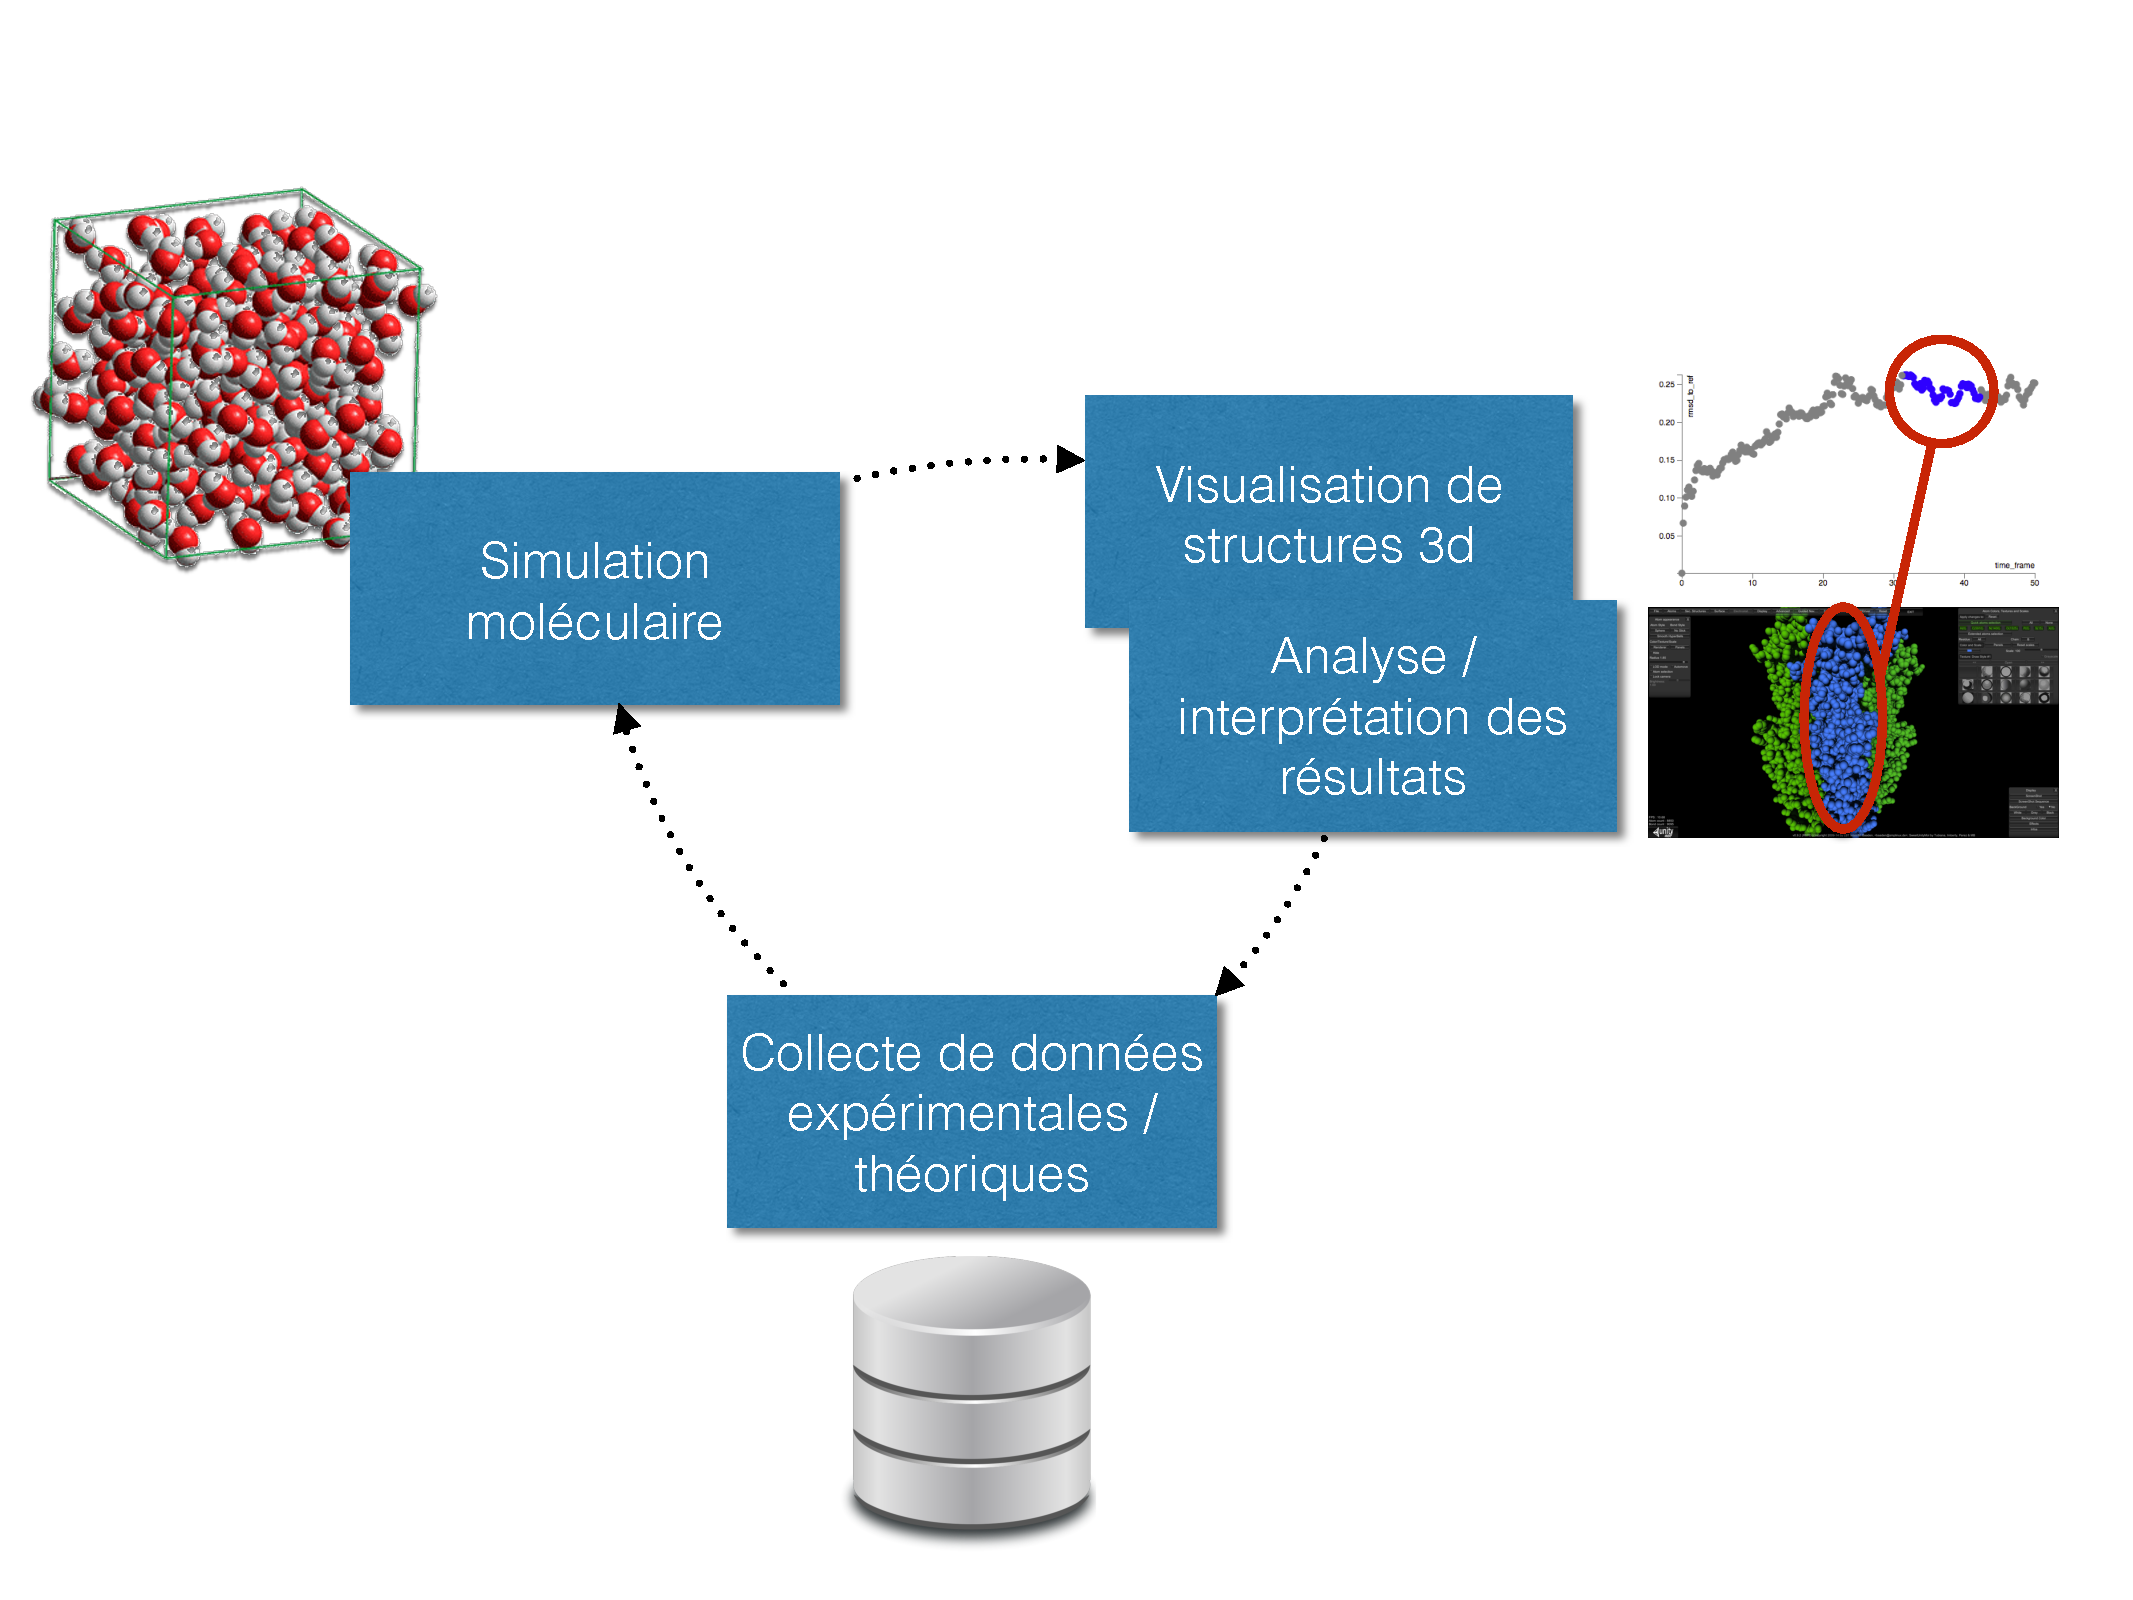
\includegraphics[width=.75\linewidth]{./figures/ch2/ch2_structural_biology_optim.pdf}}
    \caption{{\it Processus séquentiel optimisé pour l'étude d'un système moléculaire en biologie structurale.}}
  \label{Fig:schema_seq_bio_optim}
  \hspace{0.3cm}
\end{figure}


\subsection{Outils et techniques} \label{visu_ana_tools}

Plusieurs outils ou techniques découlent de ce couplage étroit entre visualisation de données brutes et analyses associées caractéristique de la visualisation analytique \cite{cockburn2008review}:

\begin{enumerate}
    \item "Overview+Detail": Cette technique met en relation plusieurs vues, synchrones ou asynchrones et dont l'une présente une vue globale du sujet,le tout dans des espaces visuels distincts. L'absence de synchronisation peut se retrouver dans la vue globale ou dans la vue détaillées. Une interaction dans l'une ou les autres des vues n'entraîne pas obligatoirement un changement dans les autres vues. Cependant, dans la plupart des cas, les vues sont synchrones et une cohérence est assurée entre les données affichées afin de pouvoir lier leur contenu. Une application connue de cette technique est retrouvée dans les programmes de visualisation de cartes comme illustré dans la Figure \ref{Fig:overview+detail}. Ces visualiseur de cartes géographiques présentent deux échelles spatiales différentes dans deux fenêtres distinctes. Seule l'interaction dans la fenêtre de contexte globale (la plus grande / principale) a un effet dans la seconde fenêtre.
    \item "Zooming": Cette technique se base cette fois sur une séparation temporelle des vues. Un zoom avant amènera une vue plus détaillée d'une scène alors qu'un zoom arrière apportera une vue plus globale. La transition entre les différentes échelles de vue peut être continue ou discrète et présenter une animation ou non. L'un des problèmes majeur de cette technique est la difficulté pour l'utilisateur d'inverser une action de zoom. En effet, la notion de défaire ou d'annuler une action en informatique fait souvent référence à des actions ayant eu pour effet de modifier l'état des données et non la vue de l'utilisateur.
    \item "Focus+Context": Cette technique permet à l'utilisateur de se concentrer sur une partie intéressante des données visualisées sans perdre le contexte global dans lequel s'inscrivent ces données. Les informations présentées dans le contexte global ne sont pas nécessairement identiques à celles présentées en détail mais les deux échelles d'information peuvent être associées à travers un affichage dynamique simple. Par exemple, si différents sets de données ont leurs entrées liées par au minimum une propriété équivalente, la sélection d'un point dans un set particulier sélectionne également toutes les points correspondants à ce point dans les autres sets. La Figure \ref{Fig:focus+context} nous montre par exemple la sélection d'un ensemble de modèles dans un set de données de simulation moléculaire. Au moment de la sélection, toutes les représentations des modèle Y dans les espaces de visualisation ou d'analyse sont également sélectionnées et visuellement mises en avant. Cet exemple spécifique d'utilisation du focus+context est appelé \textit{brush-and-link} et se retrouve dans de nombreux logiciels de visualisation des données sous forme de graphiques simples.
    \item "Cue-based techniques": Cette technique vise à mettre en avant un sous-ensemble de données intéressantes à l'utilisateur en intervenant sur la façon dont ces données sont affichées. A la différence des autres schémas décrits précédemment, elle n'intervient pas sur la taille des données mais peut être utilisé en conjonction de chacune des techniques précédentes. Elle regroupe des méthodes de brouillage visuel des données, d'ajout de labels ou de mise en place d'élément décoratifs divers pour attirer l'attention de l'utilisateur.
\end{enumerate}

\begin{figure}
  \centering
  {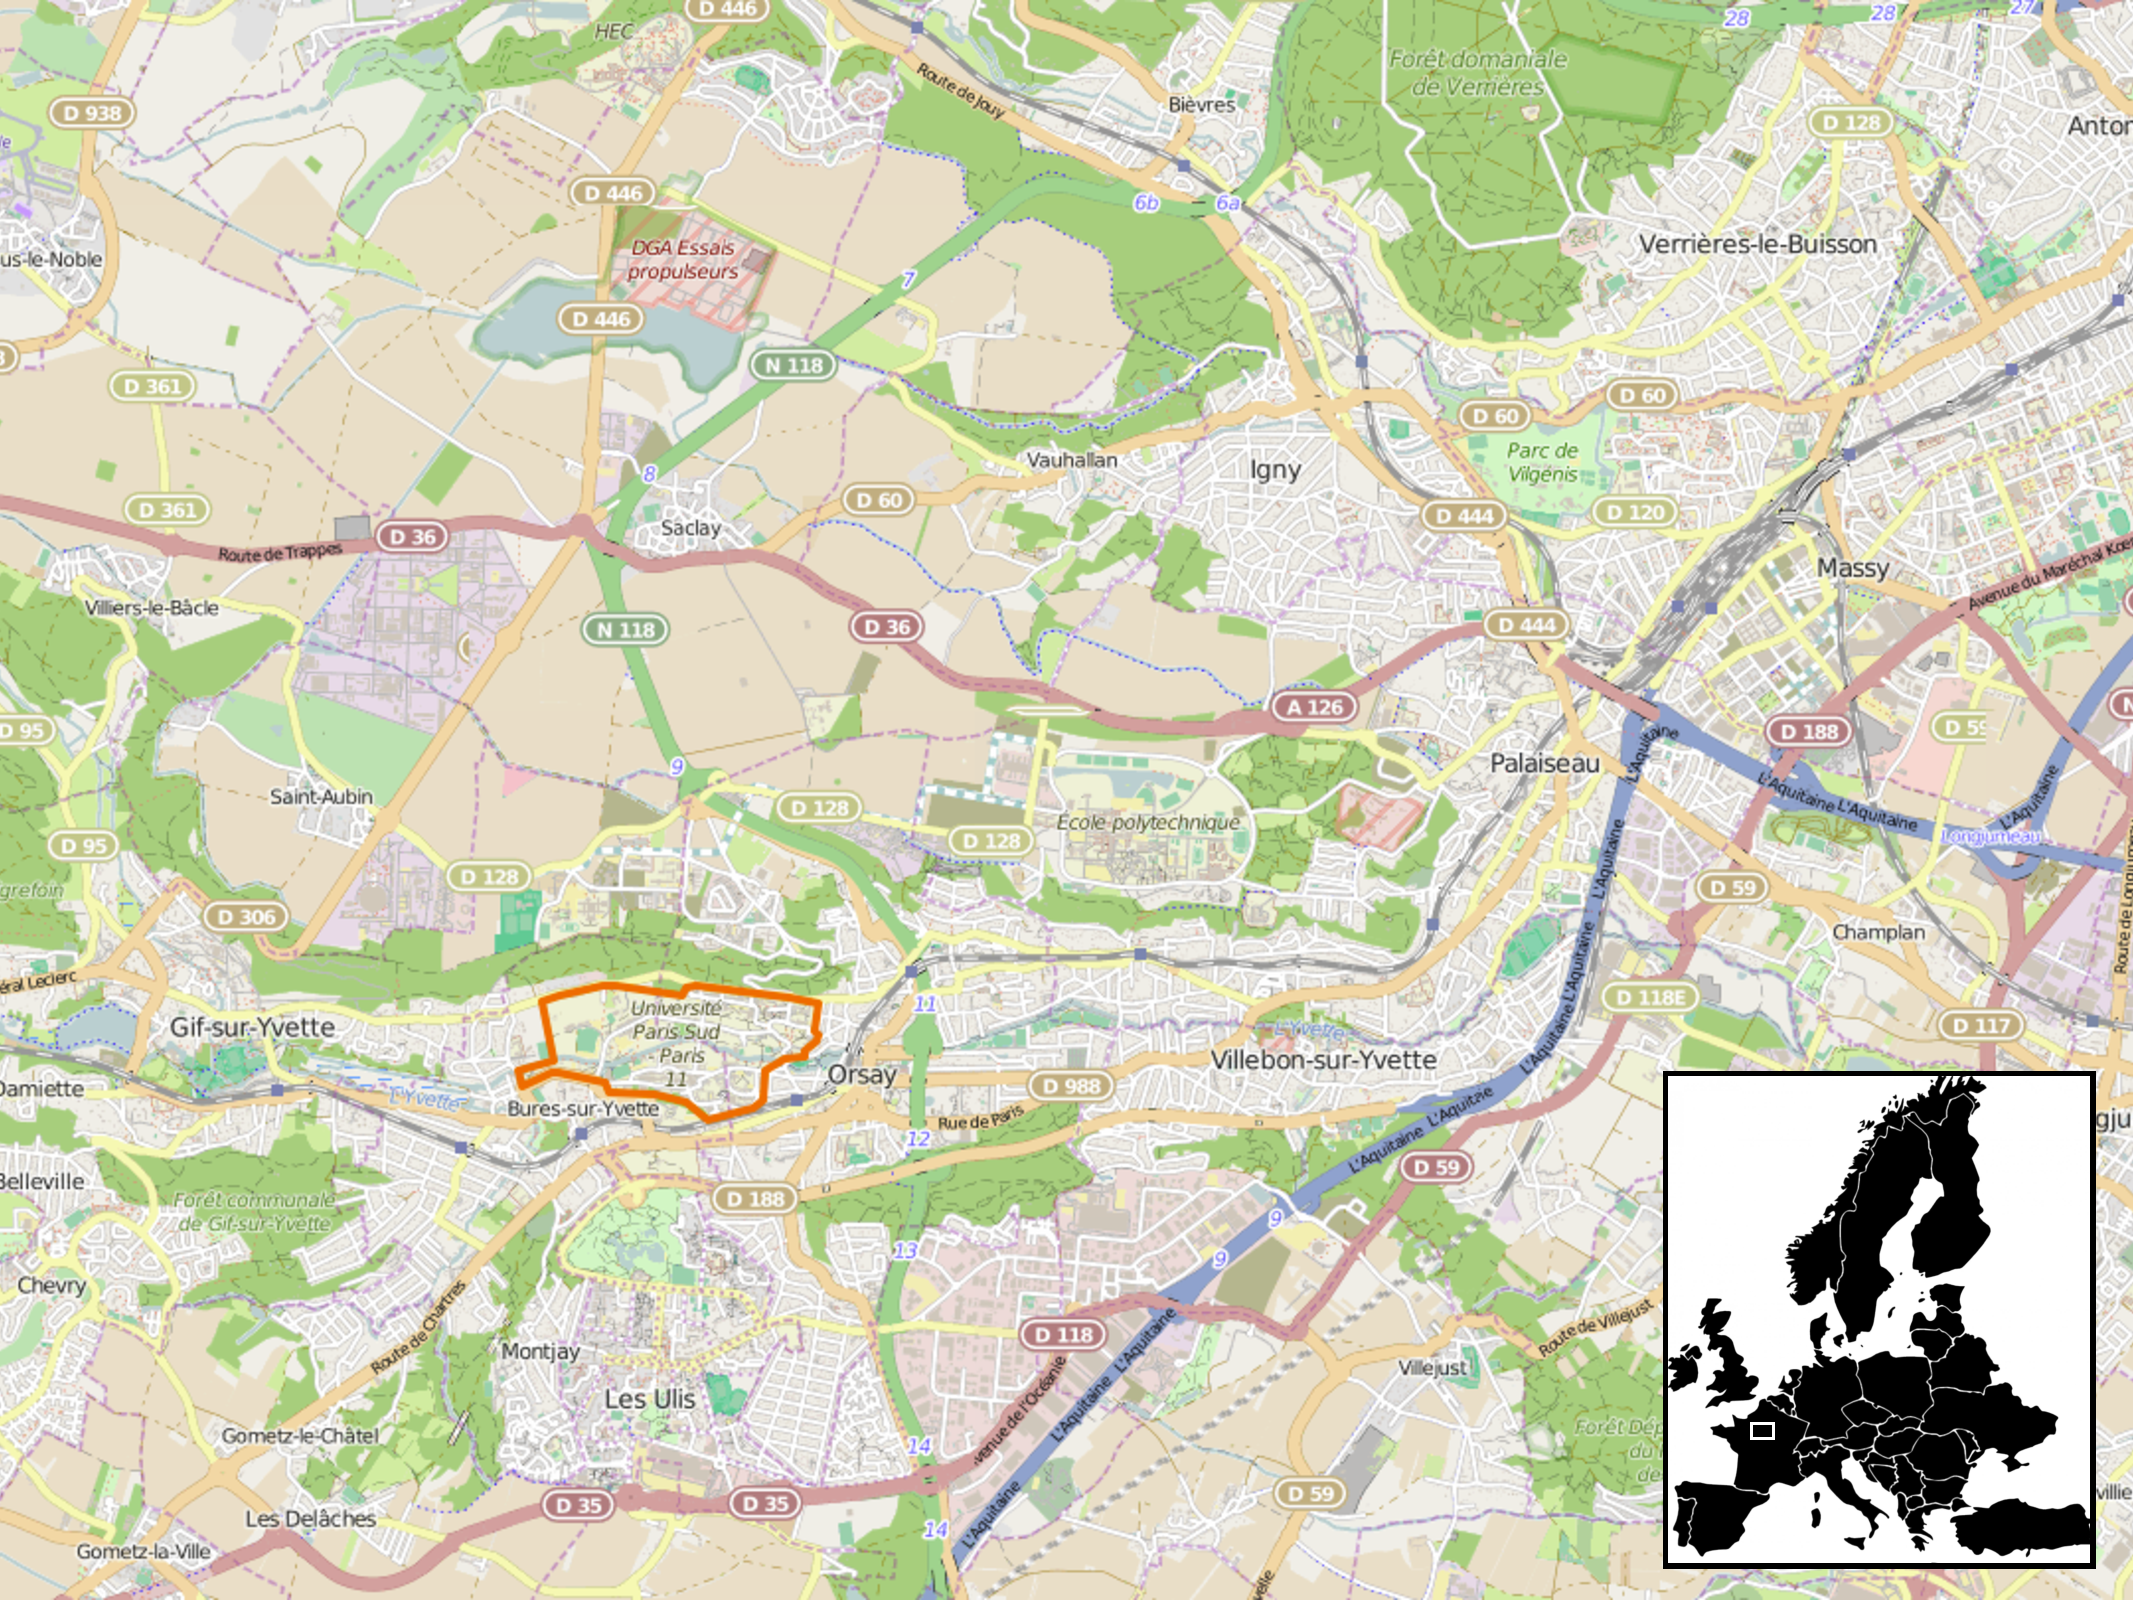
\includegraphics[width=.65\linewidth]{./figures/ch2/ch2_overview+detail}}
    \caption{{\it Exemple d'application utilisant la technique d'"Overview+Detail" où un fond de carte principal possédant une certaine concentration d'informations et ciblant une région particulière (en couleur) est mis dans un contexte plus large et moins détaillé sur un deuxième fond de carte annexe (en noir et blanc).}}
  \label{Fig:overview+detail}
  \hspace{0.3cm}
\end{figure}

\begin{figure}
  \centering
  {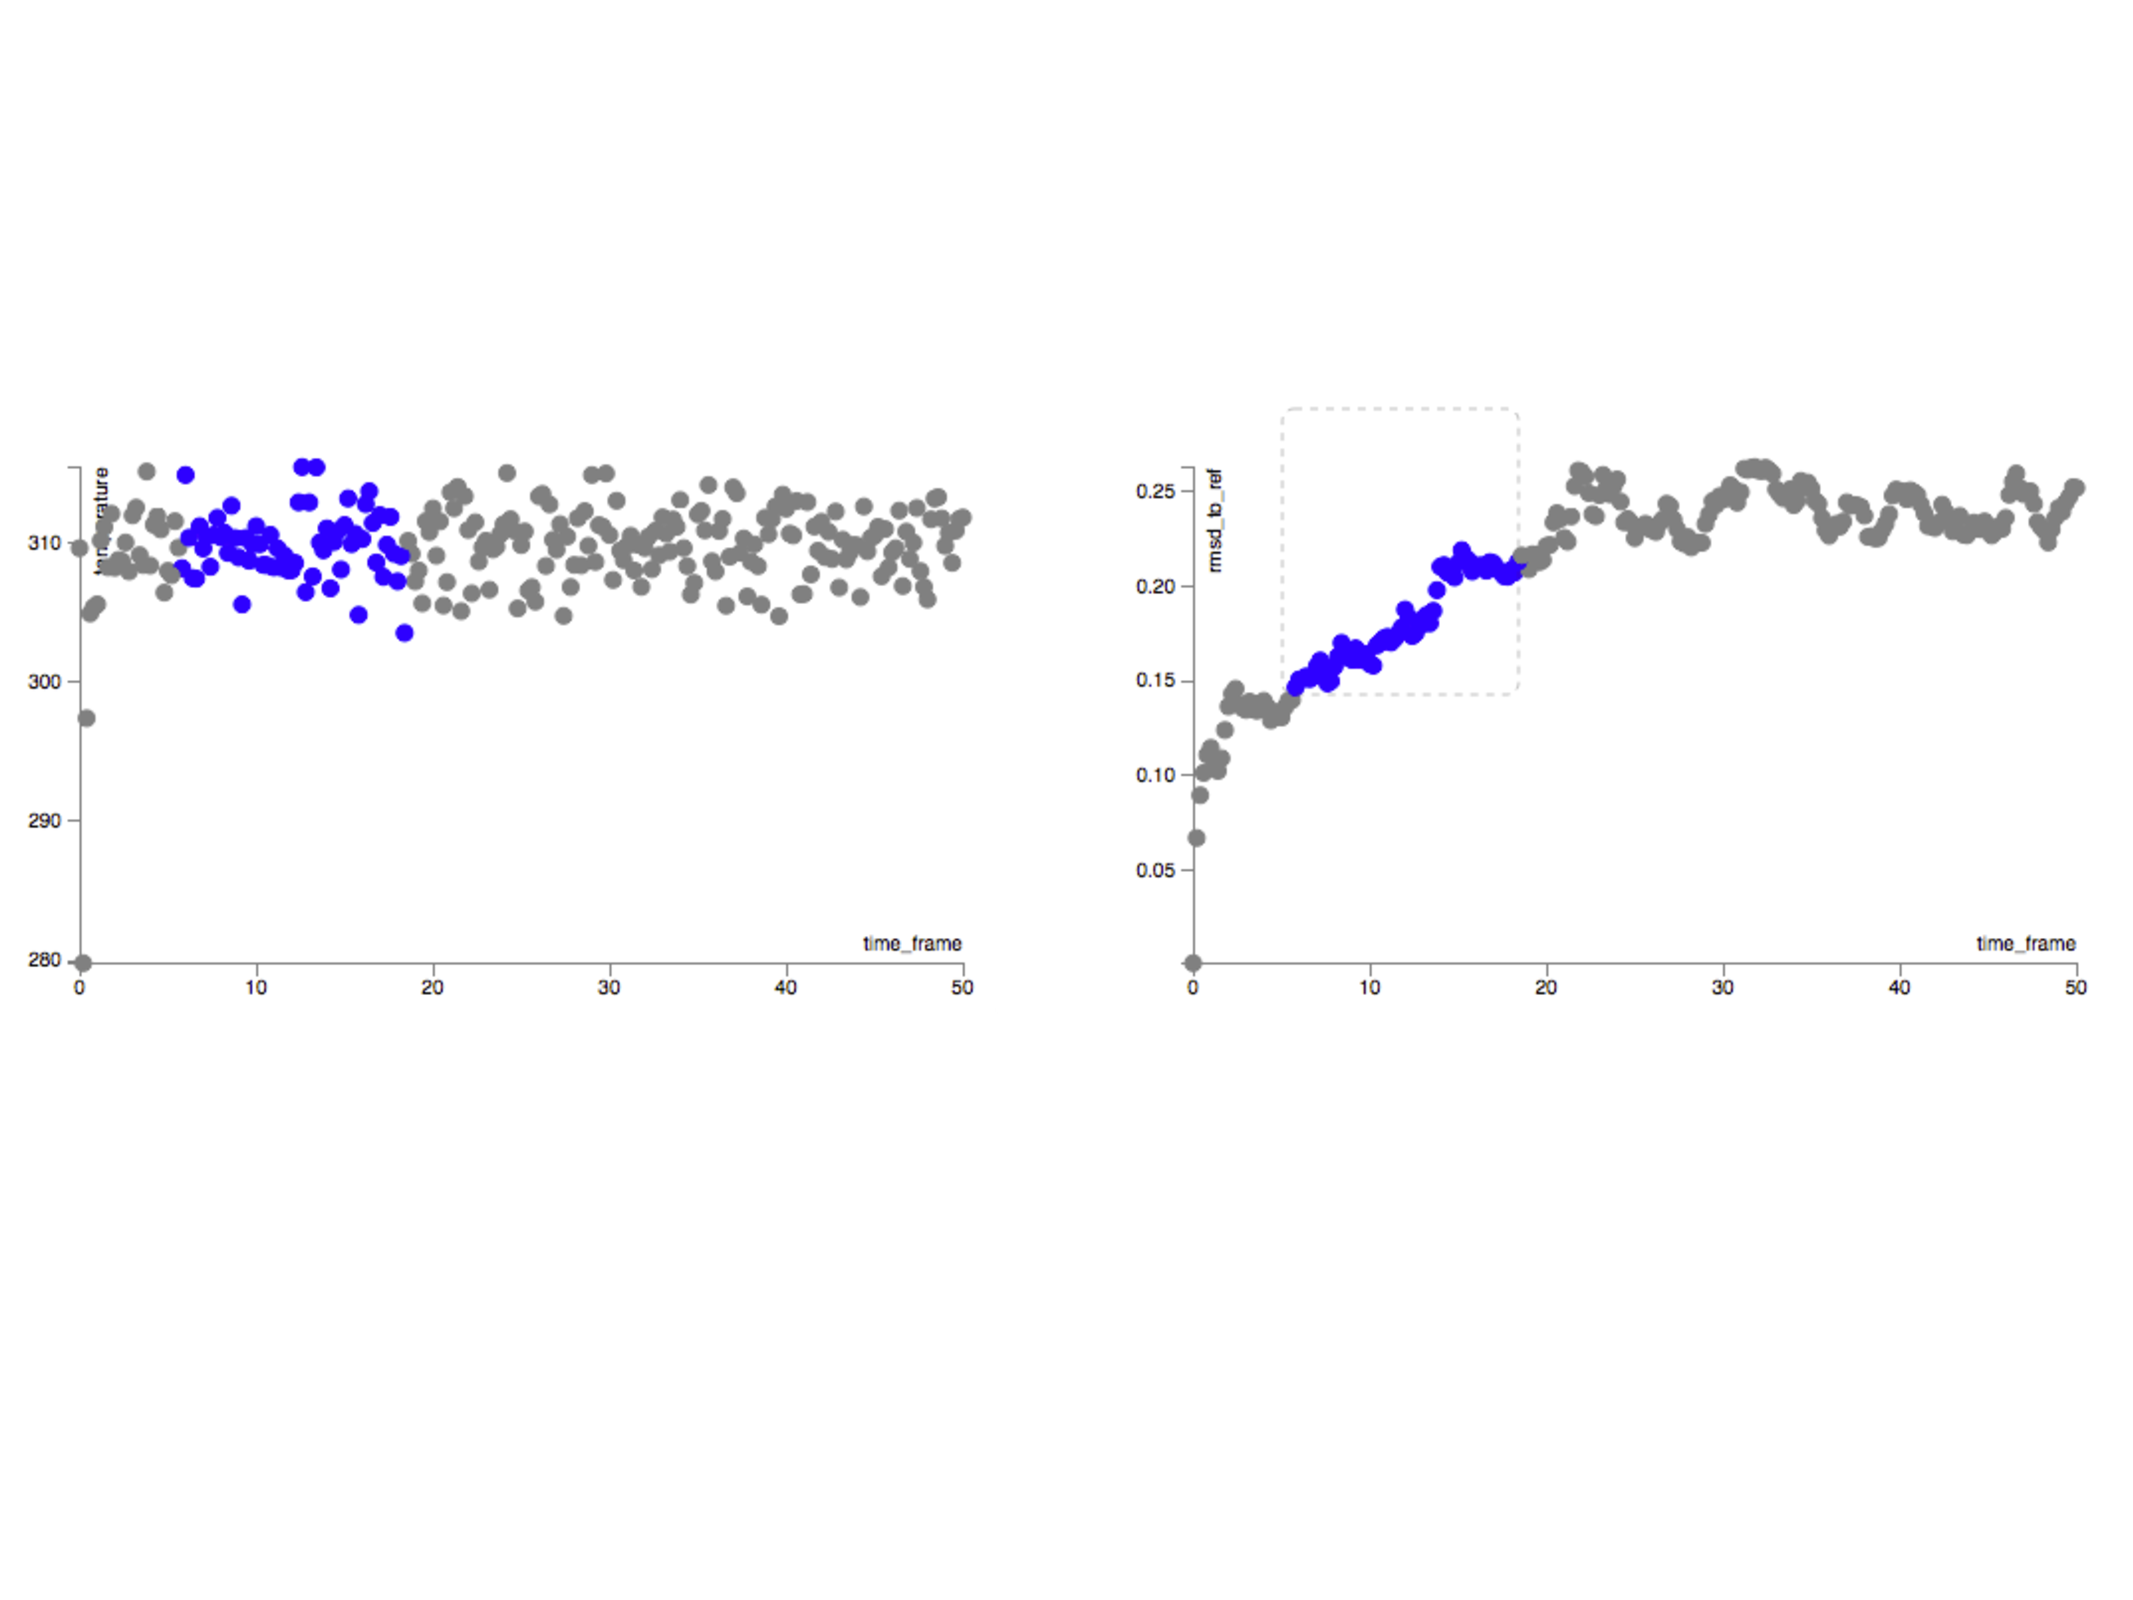
\includegraphics[width=.75\linewidth]{./figures/ch2/ch2_focus+context}}
    \caption{{\it Illustration de la sélection simultanée et synchronisée d'un ensemble d'individus dans les deux graphiques exposés. La sélection est effectuée dans le graphique de droite mais se répercute dans le graphique de gauche.}}
  \label{Fig:focus+context}
  \hspace{0.3cm}
\end{figure}


\subsection{Applications en biologie structurale}
\label{Sec:visuAnalyticsStructBio}

Bien qu'étroitement associée à de nombreuses disciplines manipulant des jeux de données de grandes tailles, la visualisation analytique n'est que partiellement utilisée en biologie structurale. La dissociation actuelle entre analyses et visualisation peut expliquer ce retard dans son implémentation au sein des outils de visualisation et modélisation moléculaire.

La visualisation analytique possède pourtant les outils nécessaires au couplage visualisation et analyses propres à l'étude d'une simulation moléculaire. En reprenant le schéma de la visualisation analytique proposé par Keim \textit{et al.} \cite{keim2010mastering}, exposé dans la Figure \ref{Fig:visual_analytics_process_keim}, il est facile de considérer la sortie d'une simulation moléculaire (des coordonnées 3D de modèles + propriétés physico-chimiques) comme données d'entrée. En utilisant des rendus visuels définis pour chaque information à observer (rendu 3D navigable pour les coordonnées 3D des complexes moléculaires, plots et graphes pour les données d'analyses, etc.) et en liant ces rendus entre-eux, il est possible de mettre en place des techniques de Focus+Context ou de Overview+Detail qui entraîneront l'adaptation synchronisée des espaces de visualisation et d'analyses \cite{schulz2011visual,kerren_toward_2012}.

On retrouve quelques caractéristiques de ce qu'apporte la visualisation analytique dans des applications comme KING \cite{chen_king_2009} ou DIVE \cite{rysavy_dive:_2014} cherchant à accroître la quantité d'informations disponibles pour l'utilisateur tout en maintenant un lien fort entre les données affichées. Une bonne présentation des informations dans leur contexte et la mise en place de connexions entre-elles apportent un environnement de décision complet pour l'utilisateur. Cytoscape \cite{shannon_cytoscape:_2003,doncheva_topological_2012} est une plateforme logicielle permettant la visualisation de réseaux complexes, notamment biologiques, associées à de nombreux types de données tels des structures 3d protéiques, graphiques d'analyses, etc.

On retrouve parmi ces derniers exemples une volonté de mettre en relation certains jeux de données afin d'en extraire des corrélations de comportement permettant de soutenir ou d'infirmer des hypothèses déjà énoncées. Cette mise en relation est possible grâce au programme utilisé, cependant, le choix des données à afficher et éventuellement à lier est le fait de l'utilisateur. Ce dernier va se servir du programme dans le seul but de faire apparaître des données de façon organisée dans le but de mettre en place des liens logiques en vue d'extraire les connaissances supplémentaires. La démarche de notre étude va plus loin puisque nous allons chercher à anticiper les éventuelles connexions entre les données afin de fournir à l'utilisateur un environnement où la majeure partie de sa réflexion ne sera pas la mise en place cognitive de ces liens mais plutôt la mise en place d'hypothèse scientifiques et l'acquisition de nouvelles connaissances. Le pré-requis de cet environnement particulier repose sur la connaissance des données et comment les présenter de façon à ce qu'une simple observation de la part de l'utilisateur lui permette de dégager une information supplémentaire, absente du champ de valeurs brutes qu'il manipule.

Il n'est pas possible de générer de tels liens entre données provenant de sources tant hétérogènes sans devoir posséder un certain niveau d'organisation et de structuration des concepts qui seront utilisés. Cette structuration peut aisément passer par une étape préliminaire de représentation des connaissances venant poser une définition et des liens ou des propriétés entre les différentes notions manipulées afin de permettre d'y appliquer un raisonnement et une certaine automatisation du rapprochement des données et de leur association aussi bien visuelle qu'organisationnelle.


% Intro sémantique / données liées
\subsection{Représentation des connaissances}

Dans les sciences informatiques, la représentation des connaissances est souvent associée à la notion d'ontologie. Une ontologie se défini comme un ensemble structuré de concepts et de relations permettant de décrire tout ou une partie d'un domaine. Une image connue énonce que "l'ontologie est aux données ce que la grammaire est au langage".

Intégrer une ontologie à un système d'information permet de déclarer formellement un certain nombre de connaissances utilisées pour caractériser les informations gérées par le système et de se baser sur ces caractérisations et la formalisation de leur signification pour automatiser des tâches de traitement de l'information.
Dans un moteur de recherche c'est, par exemple, pouvoir améliorer la recherche d'information dans sa précision, en évitant des ambiguïtés au niveau terminologique (provenant de l'homonymie) ou dans son taux de rappel, en intégrant des notions plus précises ou équivalentes (en utilisant la synonymie, l'hyponymie) ou en déduisant des connaissances implicites (par exemple, des règles d'inférence) ou en relâchant des contraintes trop strictes en cas d'échec de la requête (par généralisation) ou en regroupant des résultats trop nombreux selon leur similarité pour les présenter de façon plus conviviale (regroupement ou clustering conceptuel).

La notion de représentation des concepts et des liens entre ces concepts est connue des sciences informatiques et plusieurs formalismes en découlent. La mise en place d'ontologies afin de standardiser les connaissances dans des domaines de recherche scientifique a connu un développement spontané et important à partir de la fin des années 90 \cite{schulze-kremer_ontologies_2002, baker_ontology_1999}. 
Une ontologie est \textit{l'ensemble structuré des termes et concepts représentant le sens d'un champ d'informations, que ce soit par les métadonnées d'un espace de noms, ou les éléments d'un domaine de connaissances.}\footnote{\url{https://fr.wikipedia.org/wiki/Ontologie_\%28informatique\%29}}. Une ontologie se définit comme un vocabulaire cherchant à classer des concepts et définir des relations entre ces concepts pour un domaine spécifique. Ce classement hiérarchique se doit d'être interprétable à la fois par les machines et les humains. Tout d'abord afin d'être intégrer dans des processus informatiques et ensuite afin de servir de modèle aux scientifiques pour l'élaboration de bases de données résultantes d'ontologies.


\subsubsection{Choix du formalisme}

Afin de correctement manipuler les connaissances et les données sous-jacentes, il convient de choisir un formalisme adapté à notre objectif. Le formalisme utilisé pour représenter des connaissances dépend à la fois du domaine d'application (ici la biologie structurale), des opérations à mettre en oeuvre sur ces connaissances (lier les faits entre-eux, extraire de nouvelles connaissances, obtenir des descripteurs pertinents pour l'aide à la décision) et des processus d'implémentation qui seront utilisés (nous désirons utiliser ce formalisme au sein d'une suite logicielle multi-composants performante). Au sein des formalismes, il est possible de distinguer deux classes d'approches, les approches non logiques et les approches logiques.

Les approches non logiques regroupent des logiques descriptives comme les \textit{réseaux sémantiques} et les \textit{Graphes Conceptuels} (GC).
Les approches logiques regroupent les \textit{logiques classiques} comme la logique propositionnelle, de 1er ordre ou de 2e ordre ainsi que les \textit{logiques de description}.

\paragraph{Réseaux sémantiques}

Les réseaux sémantiques sont destinés à la modélisation hiérarchique de connaissances sous forme de graphes marqués. Un réseau sémantique contient des concepts, représenté par des noeuds et des relations, représentés par des liens (ou arcs) étiquetés entre chaque noeud. Ils ont été dans les années 60 par Quillian et Collins \cite{collins1969retrieval} comme base pour la représentation taxonomique. Ils se caractérisent par des relations binaires entre les concepts de type \textit{est-un}, \textit{a} ou \textit{type-de}.

\paragraph{Graphes Conceptuels}

Les graphes conceptuels, introduits par Sowa en 1984 \cite{sowa1983conceptual}, tiennent leur origine des réseaux sémantiques \cite{lehmann1992semantic} et sont un moyen de formaliser les connaissances \cite{chein2008graph}. Ce modèle est mathématiquement fondé sur la logique et la théorie des graphes. Cependant, pour raisonner à l'aide de GC, deux approches peuvent être distinguées : (1) considérer les GC comme une interface graphique pour la logique et donc raisonner à l’aide de la logique et (2) considérer les GC comme un modèle de représentation à part entière disposant de ses propres mécanismes de raisonnement fondés sur la théorie des graphes. Dans ce modèle, les concepts et les relations sont des noeuds reliés par des arcs orientés comme illustré dans la Figure \ref{Fig:conceptual_graph}. Les connaissances sont donc représentées par des graphes étiquetés dont les mécanismes de raisonnement se basent sur des opérations de graphes et en particulier sur l'\textit{homomorphisme} de graphes (anciennement \textit{projection}).
Un des inconvénients des GC réside dans leur faible utilisation au sein de la communauté scientifique. Peu de librairies ou applications supportant la notion de GC et la théorie des graphes qu'elle utilise existent. Leur implémentation au sein de suites logicielles en est donc partiellement difficile quand d'autres formalismes proches comportent une intégration plus importante au sein des langages de programmation les plus utilisés. De plus, ils sont exclusivement descriptifs et n'ont que peu d'extensions visées à leur adjoindre une sémantique basée sur la logique afin de pouvoir en extraire des connaissances supplémentaires.

\begin{figure}
  \centering
  {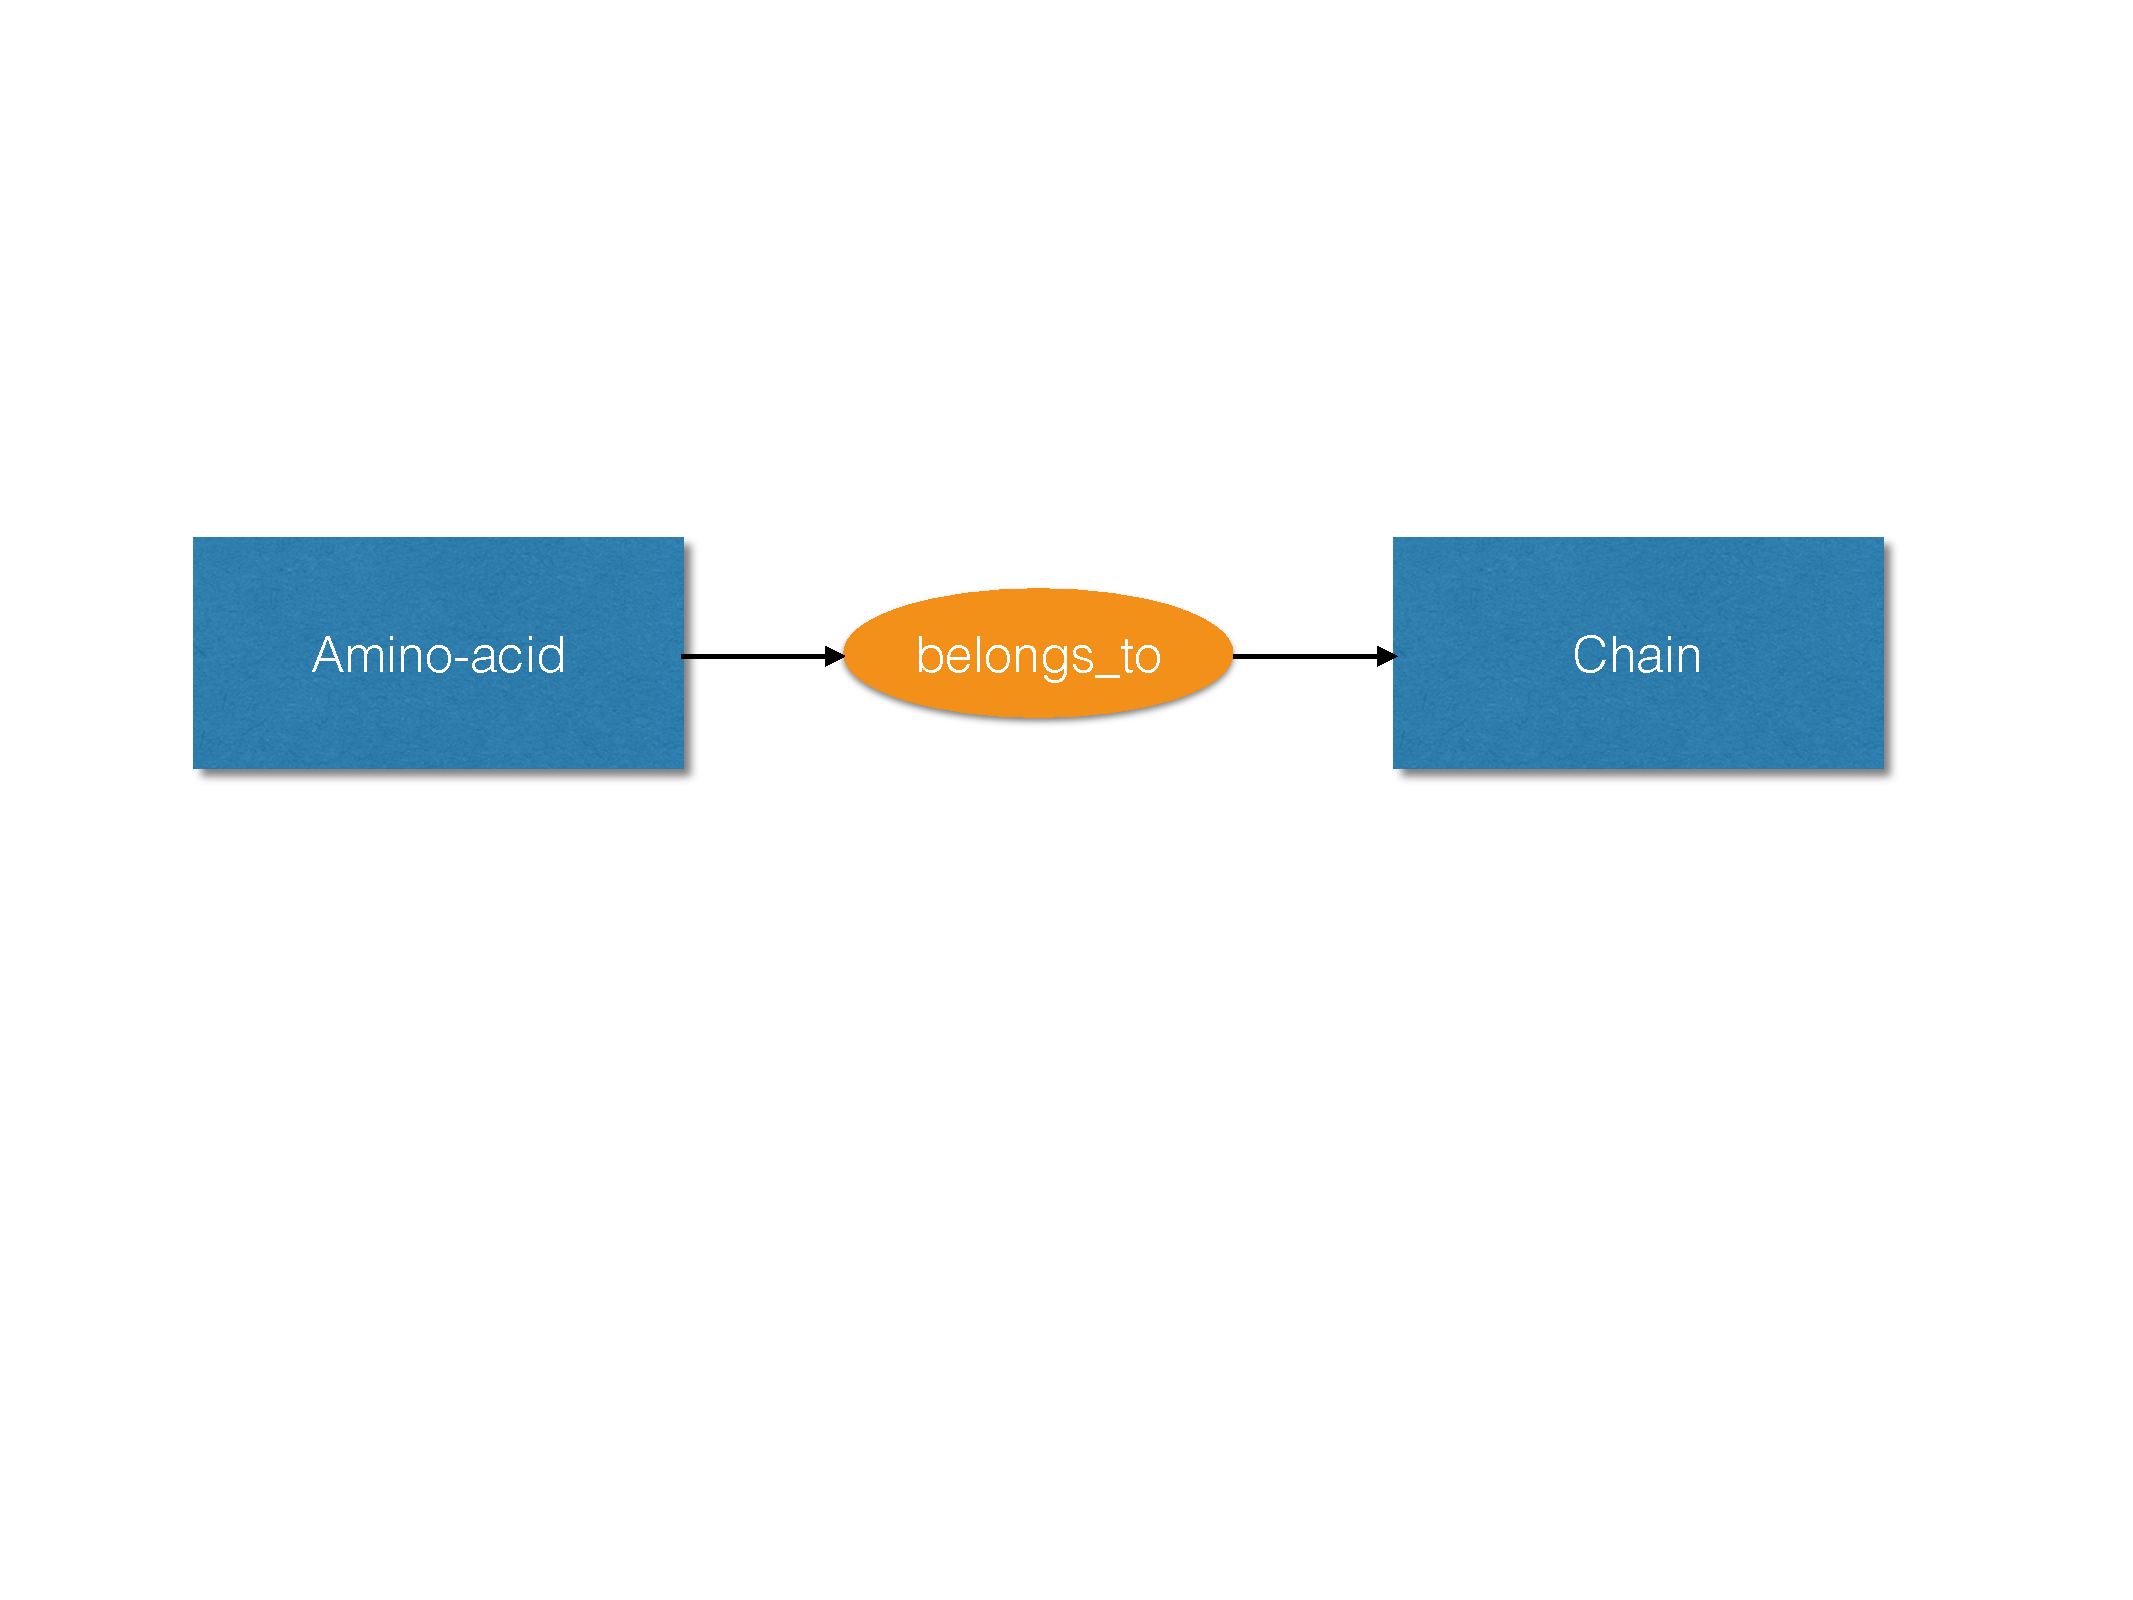
\includegraphics[width=.6\linewidth]{./figures/ch2/conceptual_graph}}
    \caption{\it Exemple de représentation sous forme de graphe conceptuel de deux concepts et une propriété. Ce sous-graphe est orienté (Ici un acide aminé appartient à une chaîne, l'inverse n'est pas vrai.) et étiqueté (les concepts sont $Amino-acid$ et $Chain$ et la propriété $belongs_to$).}
  \label{Fig:conceptual_graph}
  \hspace{0.5cm}
\end{figure}

\paragraph{Logique classique}

Les logiques de 1er ordre, 2e ordre et propositionnelles sont 3 propositions de logiques dites "classiques" présentation une première formalisation du langage et du raisonnement mathématique. Cette logique est caractérisée par des postulats qui la fondent:

\begin{itemize}
	\item Le \textit{tiers exclu} énonce que pour toute proposition mathématique considérée, elle même ou sa négation est vraie.
	\item Le \textit{raisonnement par l'absurde} qui veut prouver qu'une proposition est vraie non pas en la démontrant mais on démontrant que la proposition contraire est absurde.
	\item La \textit{contraposition} qui consiste à dire qu'une implication de type "A implique B" permet de dire que "si non-B alors non-A". B est donc une condition nécessaire de A.
	\item L'\textit{implication matérielle} ou le "seulement si" ou "si ..., alors ..." qui en logique classique se caractérise par la volonté de donner une valeur de vérité à toute proposition. Par exemple "s'il pleut, alors mon gazon est mouillé." Cette proposition ne permet pas de dire, "si mon gazon est mouillé, alors il pleut".
	\item Les \textit{lois de Morgan} qui sont des identités entre propositions logiques énonçant que "non(A et B) est (non A) ou (non B)" et "non(A ou B) est (non A) et (non B)".
\end{itemize}

Parmi les logiques classiques, la logique du 1er ordre (ou calcul des prédicats) introduit les symboles mathématiques permettant de formuler des modèles de relations au sein d'ensembles mathématiques. On retrouve dans ces symboles: Les variables, les prédicats (ou relations), les connecteurs logiques (et, ou, etc.) et deux quantificateurs universel $\forall$ ("Quel que soit", "Pour tout") et existentiel $\exists$ ("il existe au moins un ... tel que"). Les formules logiques déduites des énoncés de calculs de prédicats ont pour but de s'appliquer à n'importe quel modèle où l'on retrouve des variables, des fonctions et des prédicats représentant respectivement les éléments de l'ensemble, les fonctions de l'ensemble et les parties (ou sous-ensembles) de l'ensemble.


\paragraph{Logique de description}

Ces logiques se rapportent à la fois à la description des concepts décrivant un domaine et à la fois à la sémantique basée sur la logique. Cette logique est un apport par rapport aux réseaux sémantiques qui ne possèdent pas de sémantique basée sur la logique et sont donc exclusivement descriptives. C'est une famille de langage permettant d'une part la description des connaissances d'un domaine de façon structurée et formelle et d'autre part elles possèdent une sémantique formelle définie en logique du 1er ordre. Elles sont utilisées pour de nombreuses applications dont le web sémantique et la bio-informatique au travers d'ontologies associées au domaine. 
Similairement aux logiques classiques, les logiques de description utilisent les notions de \textit{concept}, \textit{rôle} et \textit{individu} \cite{baader2003description}. Les \textit{concepts} désignent les sous-ensemble d'élément dans un univers étudié, les \textit{rôles} correspondent aux liens entre les éléments et enfin les \textit{individus} sont les éléments de l'univers.


\subsubsection{Logiques et ontologies en biologie}

La génomique fut le domaine biologique qui a vu le premier la nécessité d'utiliser des ontologies afin d'uniformiser la quantité de données toujours plus importante générée et intégrée dans des bases de données hétérogènes à travers le monde \cite{schuurman_ontologies_2008}.
En génomique et protéomique, de nombreuses études s'appuient sur l'aide directe ou indirecte de \textit{Gene Ontology} \cite{ashburner_gene_2000}, une "bio-ontologie" qui a résulté de la prolifération de jeux de données à l'échelle génomique et la mise en place de protocoles pour l'échange et le partage de données sur le web. Elle fut le fruit de la nécessité, lors de l'explosion du nombre de données générées, de mettre en place un vocabulaire standard que les scientifiques pourraient utiliser afin de classifier et renseigner leurs données. GO n'est pas totalement considéré comme une ontologie selon la définition informatique stricte du terme car il ne possède pas de règles d'inférence complexes, ne se basant pas sur une description logique de ses concepts et sur des inférences simples de type \textit{est-un} ou \textit{est-une-partie-de}. Il est davantage mis en avant comme un vocabulaire standardisé des concepts mis en jeu dans les recherches afin de mettre en place un espace commun de termes précis et définis, possédant une hiérarchie établie. Il permet donc de mettre en relation des bases de données hétérogènes respectant ses codes ontologiques et donc d'effectuer des opérations de requêtes croisées ou de comparaison. Progressivement de nombreuses autres "bio-ontologies" sont apparues dans la lignée de GO et plusieurs d'entre-elles ont permis de mettre en avant, via le simple mécanisme d'inférence et de mise en relations des données hétérogènes, de nouvelles avancées en biologie \cite{yoshikawa_drug_2004, stenzhorn_biotop_2008, smith_obo_2007}.

Enfin, plusieurs programmes de visualisation analytique se sont appuyés sur la mise en place d'une sémantique décrivant les concepts mis en jeu \cite{rysavy_dive:_2014}. Cette représentation participe à la formalisation des concepts analysés et instaure un premier lien entre les différents modules d'un programme cherchant à partager visualisation et analyses au sein d'un même espace de travail. DIVE constitue un premier exemple de programme possédant un procédé logiciel incluant la mise en place automatique d'une ontologie afin de classer les données et de refléter le modèle de données utilisé par les librairies utilisées durant la session de visualisation et d'analyse. Le parseur mis en place dans DIVE traduit une architecture .NET \footnote{\url{https://microsoft.com/net}} en une structure de donnée hiérarchique. Chaque valeur de donnée est partagée entre l'architecture .NET et les représentations correspondantes dans DIVE permettant une modification/évolution dynamique de celle-ci pendant l’exécution du programme. Cette solution permet également de mettre en place des méthodes de requêtes sur les valeurs ou les relations entre les objets représentés et donc de mettre en avant de nouvelles informations sur les sets de données étudiés. DIVE se rapproche par plusieurs aspects de nos travaux, cependant, plusieurs points distinguent nos deux approches. Tout d'abord, afin de permettre un pré-traitement et une harmonisation des données manipulées, notre ontologie est pré-définie, imposant un contexte de travail précis et fixe. Cela favorise la mise en place de nouveaux modules car l'utilisateur sait quels concepts et propriétés sont mis en jeu dans notre processus. Comme nous l'avons fait remarquer, notre ontologie garde une certaine souplesse puisqu'il est aisément possible de l'étendre à de nouveaux concepts et propriétés suivant les besoin. Il est cependant nécessaire de garder le vocabulaire de base de l'ontologie pour pouvoir profiter de toutes les fonctions en découlant. Notre ontologie est spécifique à notre domaine d'étude, qui est la biologie structurale et plus particulièrement la visualisation et l'analyse de données de modèles de molécules dynamiques ou non. DIVE est capable de fournir une architecture plus globale puisque s'adaptant à chaque set de données mis en jeu. L'inférence propre aux ontologies est également limitée dans DIVE puisqu'elle se limite à une notion d'héritage propre au modèle OO de certains langages de programmation.


\subsection{Web sémantique et formalismes à base de graphes}


Le Web sémantique est un mouvement collaboratif mené par le \textit{World Wide Web Consortium} visant à développer des méthodes communes pour l'échange de données sur le Web. Le but du Web sémantique est de structurer et lier les connaissances présentes sur internet afin d'en faciliter le traitement et la recherche à travers le monde. Selon la définition même du W3C, \textit{le Web sémantique fournit un modèle qui permet aux données d'être partagées et réutilisées entre plusieurs applications, entreprises et groupes d'utilisateurs.} Le concept de Web sémantique n'est pas un modèle universellement adopté et, pour le moment, il se retrouve seulement dans plusieurs initiatives indépendantes attachées aux domaines de l'industrie, de la biologie et des sciences humaines. Historiquement, le Web sémantique doit ses premiers pas à Tim Berners-Lee, le directeur actuel du W3C, qui pose les premières bases d'un environnement où les données seraient classées afin de pouvoir être rapidement mises en relation et partagées \cite{berners2001semantic}. Plusieurs chercheurs ont travaillé à son utilisation et les conséquences d'un passage de l'ensemble des acteurs du web à un tel concept \cite{feigenbaum_semantic_2007}. Nous pouvons citer comme initiatives notables DBpedia, un effort pour publier les données extraites de wikipedia sous format RDF et interrogeables via SPARQL que nous décrivons ci-après \cite{auer2007dbpedia} ou le projet Data.bnf.fr\footnote{\url{http://data.bnf.fr}} qui intègre des données provenant de formats divers (Itermarc\footnote{\url{http://www.bnf.fr/fr/professionnels/f_intermarc/s.format_intermarc_biblio.html}}, XML-EAD et Dublin Core \cite{weibel1998dublin} pour la bibliothèque numérique), les regroupant et les formalisant par des traitements automatiques et les publiant dans divers standards du Web sémantique basés sur le RDF \textit{Resource Description Framework} (RDF-XML, RDF-N3 et RDF-NT, voir section \ref{rdf_model}).

Le Web sémantique se base sur un formalisme grandement inspiré des logiques de description. A l'image de plusieurs modèles du web et de l'Internet, le web sémantique est caractérisé par plusieurs couches de définition selon le schéma présenté dans la Figure \ref{web_semantic_tools}. Le modèle de graphe associé au web sémantique est le RDF \cite{klyne2006resource}. Il est structuré par le RDFS (RDF Schema) \cite{brickley2004rdf} qui décrit les vocabulaires (ontologies) sur lesquelles des ressources RDF se basent à la manière d'une DTD (Document Type Definition) pour le XML (eXtensible Markup Language) qui permet de mettre en place une hiérarchie au niveau des balises utilisée dans un document XML. 
L'ensemble des caractéristiques principales du RDFS sont repris dans un langage ontologique plus expressif appelé OWL \cite{mcguinness2004owl}. OWL fonctionne de la même manière que RDFS en étendant certaines logiques sémantiques pour le RDF. La structuration des ressources RDF avec RDFS et OWL permet l'interrogation de ces ressources par le langage de requête SPARQL (SPARQL Protocol and RDF Query Language) \cite{prud2008sparql}. RDF, RDFS, OWL et SPARQL sont tous les 4 des recommandations du W3C pour le Web sémantique et ils disposent d'une intégration de plus en plus élargie au sein des technologies et contenus web destinés au partage de connaissances et à leur traitement.

\begin{figure}
  \centering
  {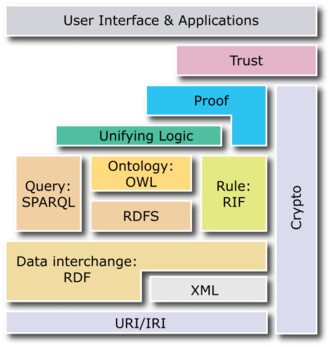
\includegraphics[width=.5\linewidth]{./figures/ch2/web_semantic_hierarchy}}
    \caption{\it Architecture du web sémantique et représentation de ses différentes couches. Cette illustration reprend notamment les standards adoptés en web sémantique et utilisés pour chaque couche d'implémentation: RDF, RDFS, OWL, SPARQL, etc..}
  \label{Fig:web_semantic_hierarchy}
  \hspace{0.3cm}
\end{figure}

\subsubsection{Modèle RDF} \label{rdf_model}

Le langage RDF est le langage de base du Web Sémantique qui l'utilise afin de mettre en place un réseau de données partagées et libres. C'est un modèle de graphe destiné à décrire de façon formelle des ressources et leurs métadonnées associées, de façon à permettre leur traitement automatique.

Le modèle RDF se base sur une représentation des connaissances à partir de triplets comme illustré dans la Figure \ref{rdf_hofstader} par Douglas R. Hofstader \cite{douglas1979godel}. Le triplet est la plus petite division de connaissances en RDF et toute description de données est un ensemble de triplets comprenant:

\begin{lstlisting}
(sujet, prédicat, objet)
\end{lstlisting}

\begin{figure}
  \centering
  {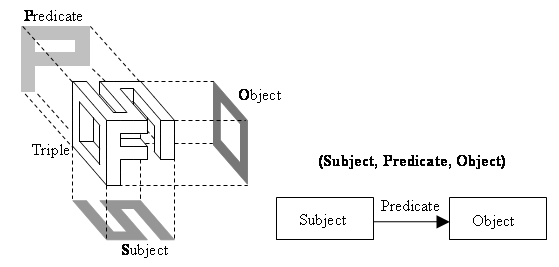
\includegraphics[width=.5\linewidth]{./figures/ch2/rdf_hofstader.png}}
    \caption{\it Illustration de la décomposition de base du langage RDF: sujet, prédicat, objet.}
  \label{Fig:rdf_hofstader}
  \hspace{0.3cm}
\end{figure}

Le \textit{sujet} représente la ressource que nous cherchons à décrire. Le \textit{prédicat} représente une propriété pouvant être associée à la ressource. L'\textit{objet} peut représenter soit une ressource, soit une donnée, cela correspond à la valeur de la propriété.
Chaque ressource est identifiée par une URI (Uniform Ressource Identifier) alors qu'une donnée est anonyme puisque pouvant être dupliquée (valeur numérique, chaîne de caractère, etc.). Un exemple de triplet pourrait être:

\begin{lstlisting}
http://mon-ontologie.fr/#Pierre 	http://mon-ontologie.fr/#âge	xsd:int^^26
\end{lstlisting}

Les ressources de ce triplet (\textit{sujet} et \textit{prédicat}) sont décris par leur URI qui est constitué d'une partie fixe (\textit{http://mon-ontologie.fr/\#}) identifiant le moyen de localiser la ressource et une partie variable (\textit{Pierre} et \textit{âge}) correspondant au nom de la ressource identifiée. Les URI les plus connues et utilisées sont les URL permettant d'accéder à des ressources internet mais les numéros ISBN référençant les livres sont également des URI. La notion d'URI est importante dans le modèle RDF car ce sont ces URI qui permettent de désigner de façon non-ambiguë une ressource que l'on souhaite décrire. Lors de la mise en place d'une nouvelle base de donnée, il est courant de créer son propre domaine de définition ou préfixe afin d'identifier toute ressource, classe ou propriété nouvelle décrite. Dans la suite de ce chapitre, nous considérerons \textit{http://mon-ontologie.fr/\#} comme notre ensemble de définition et nous le préfixerons grâce au mot-clé \textit{my}. En langage RDF, cela se caractériserait par la ligne suivante:

\begin{lstlisting}
@prefix my:    <http://mon-ontologie.fr/#>
\end{lstlisting}

La présence de cette ligne en en-tête d'un document RDF permet de réécrire l'exemple précédent:

\begin{lstlisting}
my:Pierre 	my:âge	xsd:int^^26
\end{lstlisting}

Dans des termes propres aux bases de données relationnelles SQL, RDF peut être considéré comme une table composée de 3 colonnes, sujet, prédicat, objet. A la différence de SQL cependant, la colonne objet est hétérogène et le type de donnée par cellule est sous-entendue (ou spécifié dans l'ontologie, voir \ref{rdfs}) par la valeur du prédicat.

De la même manière que les graphes conceptuels, le document RDF décrivant un ensemble de données peut être représenté par un multigraphe orienté étiqueté. Chaque triplet est représenté par un arc orienté dont les extrémités sont le sujet et l'objet et le label de l'arc correspond au prédicat. L'exemple précédent est illustré sous forme de graphe orienté ci-après:

\begin{lstlisting}
GRAPHE Pierre --âge--> 25
\end{lstlisting}

Fabien Gandon met très bien en avant le fait que le modèle RDF possède d'ailleurs plusieurs similarités avec le modèle des graphes conceptuels \cite{gandon_graphes_2008}. Ils partagent en effet la distinction entre sémantique (support pour les GC et schémas RDFS/OWL pour RDF) et la connaissance factuelle ou assertionnelle. Dans les deux modèles cette connaissance est positive, conjonctive et existentielle, pouvant être représentée par des graphes orientés étiquetés. Les schéma RDF et GC possèdent une hiérarchie similaires des classes/propriétés pour RDF et concept/relation pour GC. Les relations et propriétés sont d'ailleurs indépendantes et définies en dehors des classes/concepts et se définissent donc comme de 1er ordre dans la hiérarchie de ces deux modèles. Enfin, les deux modèles implémentent un mécanisme de déduction équivalent basé sur la subsomption en RDFS et la projection en GC. Ils s'éloignent cependant sur plusieurs points. Alors que RDF permet la multi-instanciation, GC ne possède pas d'équivalent. Une déclaration de propriété en RDF peut indiquer plusieurs domaines de définition et d'ensembles d'arrivée ce qui n'est pas le cas en GC. Les GC permettent par des relations d'arité supérieures à deux alors que les graphes RDF sont binaires. Les GC proposent également des extensions supérieures à l'expressivité de RDF/S.
Des travaux ont donc cherché à rapprocher ces deux formalismes afin de profiter de leurs avantages respectifs et gommer leurs défauts dans la mesure du possible. C'est le cas du projet CORESE \cite{corby2006searching} qui est un moteur de recherche s'appuyant sur le formalisme de RDF(S)/XML pour exprimer et partager ses données mais utilise les mécanismes de requête et d'inférence fournis par les GC. 

\paragraph{Formats et langages autour du RDF}

Les données RDF peuvent être représentées sous différents formats, du plus lisible pour l'être humain au plus optimisé pour le traitement informatique, souvent au détriment de sa lisibilité. De la même façon, ils peuvent répondre à différentes applications logicielles et donc ont été décliné également pour leur intégration dans d'autres formats courants.

La syntaxe usuelle du RDF est le XML appelé \textbf{RDF/XML}. Le format par balises du XML et les attributs associés ainsi que sa possibilité de définir des hiérarchies sont des caractéristiques du RDF/XML particulièrement appréciés pour représenter des ressources et leurs propriétés. Cette syntaxe est définie par le W3C et fut le premier standard de format pour le modèle RDF \cite{beckett2004rdf}.

Le \textbf{RDFa} (RDF dans des Attributs) est un ensemble d'éléments et d'attributs permettant d'ajouter des données RDF à des documents HTML ou XML \cite{adida2008rdfa}. Il se base sur une partie de la syntaxe HTML qu'il reprend dans l'attribut \textit{classe}, qui va préciser le type de l'objet, l'attribut \textit{id}, qu va permettre de définir l'URI de l'objet et les attributs \textit{rel}, \textit{rev} et \textit{href} qui vont spécifier des relations avec d'autres ressources. Le RDFa possède également ses propres attributs dont les plus importants sont \textit{about}, permettant d'ajouter une URI décrivant la ressource décrite par les métadonnées, \textit{property} qui va permettre d'ajouter des propriétés à la ressource décrite.

Le \textbf{GRDDL} (pour Gleaning Resource Descriptions from Dialects of Languages) est un langage, recommandé par le W3C \cite{connolly2007gleaning}, permettant d'extraire des données RDF depuis un document XML ou XHTML grâce à des algorithmes de transformation et peut fonctionner comme implémentation du XSLT (Extensible Stylesheet Language Transformations, langage de transformation du XML en formats plus lisibles comme l'HTML, le PDF ou le PNG par exemple).

La \textbf{Notation3} ou \textbf{N3} est une norme de sérialisation non-XML pour le modèle RDF. Elle a été mise en place afin de fournir une syntaxe plus compacte et plus facile à lire. Elle a été développé, entre autres, par Tim Berners-Lee au sein de la communauté du Web sémantique \cite{berners2008n3logic}. La norme N3 est davantage qu'une norme de sérialisation pour RDF puisqu'elle supporte également les règles basées sur RDF. Elle permet l'utilisation de symboles spécifiques pour éviter la répétition de motifs communs entre les triplets. Par exemple:

\begin{lstlisting}
my:Alanine	rdf:type 	my:Acide-aminé ; 
	my:a-une-charge		my:Positive ; 
	my:est-composé-de 	my:Carbon_alpha, my:Carbon_beta	
\end{lstlisting} 


Ici le ";" est utilisé afin de conservé le sujet (<Alanine>) alors que la "," est elle utilisée pour conservé le sujet et le prédicat (<Alanine> et my:est-composé-de).

Le \textbf{Turtle} est un sous-ensemble de la syntaxe N3 n'existant pour le moment que sous forme de recommandation du W3C \cite{prud2013turtle}. Sa majeur différence avec le N3 est syntaxique. Il se rapproche beaucoup du format utilisé dans le langage de requête SPARQL (voir \ref{sparql}).

\textbf{N-Triplet} est un autre sous-ensemble de N3 beaucoup plus explicite puisque ne comportant pas de symboles particuliers simplifiant les descriptions de ressources. Son utilisation se limite souvent aux jeu de données RDF relativement restreints car son traitement a un coût computationnel assez élevé et la taille des fichiers générés est conséquente.

\textbf{JSON-LD} (ou JavaScriptObjectNotation for Linked Data) est une méthode de transmission des données liées RDF basée sur JSON. Pour rappel, JSON est un format standard ouvert largement utilisée dans les protocoles de communication asynchrones entre serveurs et clients web. Il se base sur la déclaration de structures clé/valeur, particulièrement adaptées à la description de concepts. 
Dans le cadre de JSON-LD, les clés sont les propriétés du concept, associées à leur valeur. Les valeurs peuvent être des références à d’autres concepts, des nombres ou encore du texte simple\footnote{\url{http://www.woptimo.com/2015/02/json-ld-la-revolution-semantique-des-microdonnees/}}. Deux propriétés sont obligatoires, \textit{context} et \textit{type}, et définissent respectivement l'ontologie utilisée et le meta-concept du concept courant (la ressource décrite). Un exemple de document JSON-LD est présenté ci-dessous:

\begin{lstlisting}[language=XML]
<script type="application/ld+json">
{
	"@context": "http://schema.org/",
	"@type": "Movie",
	"name": "Brannigan",
	"genre": "Thriller",
	"trailer": "https://www.youtube.com/watch?v=gAhzli9jbKU",
	"actors":
		{
		"@type": "Person",
		"name": "John Wayne",
		"birthDate": "1907-05-26"
		}
}
</script>
\end{lstlisting}

JSON-LD tend à devenir la nouvelle norme, majoritairement grâce à son interaction avec les bases de données, en particulier NoSQL. Le domaine du \textit{Big Data} connaît un essor exponentiel et beaucoup de grands acteurs du web (Google, Amazon, Twitter, etc.) migrent vers des paradigmes NoSQL, plus rapides. Les API qu'ils mettent à disposition sont accessibles à travers le protocole HTTP et utilisent le format JSON pour communiquer. Trois raisons principales pour l'utilisation de ce format: Sa compréhension aisée, sa structuration et son faible poids. L'ajout d'une couche sémantique avec JSON-LD en est donc grandement facilitée. 

Nous avons vu que le modèle de représentation RDF s'appuie sur un formalisme précis et standardisé qui permet l'uniformisation des données représentées et la mise en place de lien entre ces données. Ce formalisme n'est qu'une méthode de représentation et ne constitue pas une logique de raisonnement qui permettrait d'extraire des connaissances de ces données. C'est dans ce but qu'a été créé RDFS et OWL, des langages formels servant à décrire des ontologies. A la différence des données RDF qui sont de l'ordre du \textit{factuel}, une ontologie permet de décrire les concepts et les relations entre ces concepts et constitue la partie \textit{structurelle} du Web sémantique.
OWL et RDFS reprennent les critères standards des ontologies existantes et qui est le support de nombreuses ontologies recensées dans le portails officiels de bio-ontologies largement utilisées dans la communauté scientifique \cite{smith_obo_2007}.

\subsubsection{RDF Schema} \label{rdfs}

RDFS fut la première extension permettant d'ajouter une couche sémantique au modèle de ressource RDF. Il définit les notions de classes, sous-classes, propriétés et sous-propriétés desquelles dépendront les ressources RDF identifiées. C'est donc un ensemble de concepts haut-niveau définissant les différents individus d'un domaine et permettant leur hiérarchisation. 
Par exemple, RDF permet de décrire qu'une <Lysine> \textit{a une charge} <positive> grâce aux individus <Lysine> et <positive>, respectivement sujet et objet, et au prédicat \textit{a une charge}. RDFS permet d'ajouter les concepts décrivant les individus comme <Acide-aminé>, <Charge>, <Hydrophobicité>, <Molécule>, etc. et de préciser des relations entre ces groupes de façon à pouvoir émettre des déductions simples. Par extension de l'exemple précédent, si l'on ajoute que tout <Acide-Aminé> est une <Molécule> qui revient à dire en RDFS, <Acide-aminé> \textit{sous-classe de} <Molécule>, et <Lysine> \textit{instance de} <Acide-aminé>. Cela nous permet d'ajouter un niveau d'information induite des deux affirmations précédente qui serait: <Lysine> \textit{instance de} <Molécule>. Cette déduction se fait grâce au système d'implication introduit par RDFS et permettant de déduire des informations complémentaires à partir d'un minimum de données.

RDFS introduit également la notion de domaine de définition (\textit{rdfs:domain}) et d'ensemble d'arrivée (\textit{rdfs:range}) pour les propriétés. Le domaine de définition correspond à la classe des sujets liés à une propriété alors que l'ensemble d'arrivée correspond à la classe ou au type de données des valeurs de la propriété. Il est par exemple possible de préciser que la propriété <identifiant> doit avoir comme domaine de définition seulement des individus de classe <Objets> et comme ensemble de définition des valeurs de type <xsd:integer>.
Le système d'implication de RDFS fonctionne également avec les notions de domaine d'application et d'ensemble de définition. De ce fait, ces 3 affirmations:

\begin{lstlisting}
<my:Alanine>	<my:est-un>		<my:Acide-aminé> .
<myProtéine>	<my:contient>	<my:Lysine> .
<my:contient>	<rdfs:range>	<my:Acide-aminé> 
\end{lstlisting}

permettent d'induire l'affirmation suivante:

\begin{lstlisting}
<my:Lysine>		<my:est-un>		<my:Acide-aminé>
\end{lstlisting}

\subsubsection{OWL} \label{owl}

OWL est donc un standard informatique visant également à jouer le rôle de grammaire pour le langage RDF en complément du RDFS à qui il reprend ses bases. Le langage OWL se base sur des éléments des logiques de description et constitue un standard informatique permettant de vérifier que les données soient cohérentes, de déduire de nouvelles connaissances de ces données ou d'en extraire certaines informations.
Plus expressif que RDFS, OWL permet d'adjoindre à la définition des relations entre objets par des assertions fournie par RDFS, des propriétés reliant les classes à travers des relations de symétrie, d'équivalences, de cardinalité, etc. entre les classes. 
Il est donc possible de mettre en place des associations de classes et de propriétés plus complexes et basée sur une fondation logique  

Si l'on étend l'exemple précédent avec les notions apportées par OWL au sein des triplets suivants:

\begin{lstlisting}
<est-composé-de> \textit{est} <owl:TransitiveProperty>,
<Protéine> <est-composé-de> <Acide-aminé>,
<Acide-aminé> <est-composé-de> <Atome>
\end{lstlisting}

nous pouvons donc en déduire, grâce au caractère transitif de la propriété <est-composé-de>, que:

\begin{lstlisting}
<Protéine> <est-composé-de> <Atome>
\end{lstlisting}

De la même manière, il est possible de définir des propriétés comme symétriques, asymétriques, inverses, réflexives, etc.\footnote{\url{http://www.w3.org/2007/OWL/wiki/Quick_Reference_Guide}}
OWL est composé de 3 sous-langages classés du moins expressif au plus expressif: OWL-Lite, OWL-DL et OWL-Full. Parmi ces sous-langages, seul OWL-Lite est implémenté sous forme d'algorithmes décidables dans la majorité des moteurs d'inférence utilisé lors de l'interrogation de bases de données RDF possédant une ontologie OWL associée. La simplicité d'OWL-Lite lui permet une complexité réduite et donc un temps de calcul également réduit lors de son utilisation. Il regroupe les principales relations et descriptions de classe amenée par OWL et permet ainsi une mise en place de logiques descriptives suffisamment évoluées pour permettre l'extraction de nouvelles connaissances à partir de données simples.

\subsubsection{SPARQL} \label{sparql}

Nous venons d'évoquer la possibilité d'utiliser un moteur d'inférence afin d'extraire des données d'une base de données RDF. Cette extraction peut se faire via l'utilisation d'un protocole et langage de requête appelé SPARQL. Ce langage permet à la fois de récupérer des données stockées sous format RDF dans une base de données mais également de les éditer, d'en ajouter ou bien d'en supprimer. L'accès aux bases de données se fait grâce à une interface d'accès (en anglais \textit{endpoint}) géré par un service capable de recevoir des requêtes SPARQL et de renvoyer des résultats sous différents formats.
A la différence du SQL, SPARQL se base essentiellement sur le format en triplets des bases de données RDF et la majorité de ses requêtes repose sur la mise en place d'un schéma de correspondance entre triplets sujet/prédicat/objet. Il n'y a pas de contraintes de typage pour la colonne objet qui est habituellement implicite ou définie par l'ontologie. Dans le même esprit, l'ontologie est directement intégrée dans les résultats de requêtes et le schéma de données n'a donc pas besoin d'être appliqué de façon séparée. SPARQL fournit également plusieurs opérations sur les résultats comme SORT, JOIN, DISTINCT, qui permettent un traitement direct des résultats afin de les classer ou filtrer suivant les besoins...\footnote{\url{http://www.cambridgesemantics.com/semantic-university/sparql-vs-sql-intro}} Certains mots-clés de SQL ont été conservé tels que SELECT, FROM, WHERE, etc.
Une requête SPARQL se retrouve sous la forme suivante:

\begin{lstlisting}[language=SPARQL]
SELECT ?x ?id
FROM <http://my\_database.com> 
WHERE {
	?y my:est-composé-de ?x .
	?y rdf:type my:Chain .
	?y my:chain\_id "B" .
	?x my:res\_id ?id
}
\end{lstlisting}

Dans son fonctionnement, SPARQL va effectuer deux opérations successives sur la base de données. Une première étape est la recherche des triplets correspondant au modèle de triplet énoncé dans la requête. C'est l'étape de restriction qui va retourner l'ensemble des lignes de la base de données construits sur ce motif et comportant les valeurs spécifiées quand elles le sont (ici \textit{my:a-une-charge}, \textit{my:positive} et \textit{my:res\_id}). Cette étape se rapporte donc à ce qui se trouve dans le "WHERE". Lorsque les triplets sont identifiés, SPARQL va sélectionner uniquement les variables demandées au niveau du mot-clé "SELECT", ici ?x et ?id. C'est l'étape de projection qui va venir sélectionner les colonnes que l'utilisateur a demandé parmi les lignes sélectionnées dans l'étape précédente. Le résultat de la requête SPARQL précédente sur le jeu de données fourni en Annexe A pourrait donc être:

\begin{center}
 \begin{tabular}{|c | c|} 
 \hline
 ?x & ?id \\ [0.5ex] 
 \hline
 RES\_11 & 1 \\ 
 RES\_12 & 2 \\
 RES\_13 & 3 \\
 RES\_14 & 4 \\
 RES\_15 & 5 \\
 \hline
\end{tabular}
\end{center}

Les résultats sont présentés par défaut sous forme de tableaux par soucis de clarté mais la plupart des services SPARQL permettent leur conversion automatique en un nombre important de formats comme le XML, le JSON, Javascript, Turtle, etc.
De nombreuses librairies utilisent des points d'accès SPARQL afin d'y présenter des requêtes et d'en récupérer leurs résultats. Cette implémentation présente dans de nombreux langages de programmation assure une certaine généricité du travail d'interfaçage nécessaire dans une suite logicielle multi-composants.

\subsection{Implémentations et outils} \label{web_semantic_tools}

Nous avons évoqué la présence de librairies ou plateformes implémentant les standards du web sémantique et permettant d'utiliser ce modèle de représentation de données pour des activités hétérogènes. Nous pouvons citer plusieurs d'entre-eux, associés fortement au web sémantique et cherchant à se développer parallèlement au domaine afin de lui offrir un support aussi complet que possible. Parmi ceux-ci:

\begin{itemize}
	\item \textbf{Jena}\footnote{\url{https://jena.apache.org/index.html}} \cite{jena2007semantic} est l’un des moteurs actuels les plus complets et propose une persistance en mémoire ou en base de données. C'est une structure logicielle Java gratuite et ouverte implémentant RDF, RDFS et OWL ainsi que les requêtes SPARQL et propose un moteur en chaînage avant (RETE), arrière (programmation logique) et hybride. Ce moteur est utilisé pour implanter la sémantique de RDFS et OWL et son modèle repose sur une structure prédéfinie de bases de données.
	\item \textbf{Protégé}\footnote{\url{http://protege.stanford.edu/}} \cite{noy2001creating} est un outil basé sur Java et utilisé pour construire et éditer des ontologies. Il supporte RDF et OWL de façon native et intègre différents outils comme un visualiseur de réseau ontologique sous forme de graphe orienté ou une interface de requête SPARQL. Il est capable d'utiliser certains moteurs de logique de description afin d'inférer une ontologie ou de la valider.
	\item \textbf{Corese}\footnote{\url{http://wimmics.inria.fr/corese}} \cite{corby2006searching} est un moteur de recherche basé sur l'ontologie et rapprochant les approches de graphes conceptuels et de RDFS afin de répondre à des requêtes faites sur des annotations RDF. Il étend ainsi les règles d'inférence RDFS en s'appuyant sur certaines opérations propres aux graphes conceptuels.
	\item \textbf{Triple} \cite{sintek2002triple} est un langage de requêtes basé sur la logique de Horn permettant d'interroger des données du web sémantique et principalement des données RDF. Il est capable de raisonner grâce à des moteurs d'inférence et intègre les primitives RDF comme les espaces de nommage, les ressources et la notion d'individu (à opposer à concept ontologique). Son principal atout réside dans sa capacité à interroger différents modèles de données grâce à différentes logiques de description.
	\item \textbf{Fact} et son successeur \textbf{Fact++} \cite{tsarkov2006fact++} est un moteur à base de logiques de descriptions permettant de générer des requêtes conjonctives qui vont identifier, classifier ou valider des données d'une base de connaissances à partir de son ontologie. Ce moteur est à même de comprendre les ontologies OWL et donc d'appliquer les règles d'inférences qui lui sont associés. Il est par exemple implémentable dans l'outil Protégé cité précédemment.
\end{itemize}


\section{Perspectives en RV et VA pour la biologie structurale} % (fold)
\label{sec:perspectives}

Nous avons souligné dans la section \ref{RV_science} les caractéristiques de la RV et ce qu'elle pouvait apporter à l'expérience de travail. A savoir qu'au-delà d'un simple rendu stéréoscopique, les enjeux d'une implémentation réussie en RV passe par la mise en place d'interactions adaptées et pertinentes pour la tâche experte prévue.

Parmi les problématiques soulevées par la RV pour les données abstraites et scientifiques, nous avons déjà évoqué le cantonnement de la discipline à des tâches d'exploration et de visualisation de structures 3d. La réalisation de tâches nécessitant une certaine interaction avec les données mises en jeu, dans un premier temps exclusivement 3d, nécessite la mise en place de méthodes de navigation adaptées. Or la navigation au sein des mondes virtuels est l'un des obstacles cruciaux à franchir pour assurer une expérience optimale aux utilisateurs. En effet, la notion de monde virtuel implique la possibilité pour l'utilisateur d'évoluer au sein d'un environnement étendu de la même manière qu'il évoluerait dans la vie réelle. Or, si cette navigation virtuelle peut être approchée par le biais de la navigation réelle dans le cas d'environnements virtuels écologiques, là où le contenu virtuel proposé est une copie artificielle d'éléments réels, la question est toute autre lorsque la scène observée n'est plus écologique et implique des éléments abstraits. Le degré d'abstraction, important en biologie structurale, décidera directement de la quantité de repères spatiaux dont l'utilisateur disposera pour naviguer. La visualisation moléculaire met en scène des représentations artificielles d'atomes, non observables à l’œil humain en temps normal, et dont les couleurs et formes respectent des standards décidés par la société mais non dictés par des observations réalistes. Les repères spatiaux sont donc peu nombreux et souvent trop sommaires pour assurer une orientation acceptable de l'utilisateur. Afin de combler ce manque préjudiciable pour l'expérience utilisatrice lors de ses futures tâches en biologie structurale, nous avons développé une série de paradigmes de navigation, basées sur le contenu observé et les tâches usuelles en visualisation/exploration moléculaire.

Dans la même optique de mettre en place un environnement virtuel respectant les contraintes de la RV, il nous a paru important d'adapter les interactions habituelles qu'un expert peut avoir dans des sessions de visualisation et d'analyses. Ces interactions, trop complexes et trop cloisonnées dans des environnements de bureau, doivent être simplifiées et harmonisées afin de pouvoir faire cohabiter et communiquer les étapes complémentaires que sont la visualisation et l'analyse. On remarque que dans la boucle de la VA (voir Figure \ref{Fig:visual_analytics_process_keim}), ces deux étapes sont très proches, aussi bien en terme de données utilisées que d'implication de l'utilisateur. Leur rapprochement et fusion au sein d'un unique module est donc relativement pertinent et pourrait donc se faire via la mise en place d'une représentation des notions utilisées dans chacune des étapes. L'utilisation d'ontologie comme illustré précédemment permet cela et va même plus loin car elle pourrait simplifier l'étape de \textit{transformation} des données en imposant un carcan et un vocabulaire précis aux données d'entrée. Ce deuxième pan de notre étude nous a mené à la mise en place d'une plateforme multi-composants s'appuyant sur l'utilisation d'une base de données RDF dont la structure dépend directement d'une ontologie OWL créée pour décrire notre domaine d'application.


% section probl_matique (end)